%%%%%%%%%%%%%%%%%%%%%%%%%%%%%%%%%%%%%%%%%
% Focus Beamer Presentation
% LaTeX Template
% Version 1.0 (8/8/18)
%
% This template has been downloaded from:
% http://www.LaTeXTemplates.com
%
% Original author:
% Pasquale Africa (https://github.com/elauksap/focus-beamertheme) with modifications by 
% Vel (vel@LaTeXTemplates.com)
%
% Template license:
% GNU GPL v3.0 License
%
% Important note:
% The bibliography/references need to be compiled with bibtex.
%
%%%%%%%%%%%%%%%%%%%%%%%%%%%%%%%%%%%%%%%%%

\documentclass{beamer}

\usepackage{graphicx}
\usepackage{subcaption} %to have subfigures available

\pdfminorversion=5
\usefonttheme{structuresmallcapsserif}
\usetheme{focus}

\vspace{-50pt}
%\title{Thesis Defense}
\title{Scalable Processing of \\Moving Flock Patterns}
\subtitle{}

\author{
    Andres Calderon \textperiodcentered \ acald013@ucr.edu \\
}

\institute{University of California, Riverside}

\begin{document}
    \begin{frame}
        \maketitle
    \end{frame}

%     \begin{frame}{Outline}
%         \begin{itemize}
%                 \item Scalable overlay operations over DCEL polygons layers
%                 \item Towards parallel detection of movement patterns in large trajectory databases
%         \end{itemize}
%     \end{frame}
%
%     \begin{frame}{Outline}
%         \begin{itemize}
%                 \item \textbf{Scalable overlay operations over DCEL polygons layers (SSTD'23)}
%                 \item Towards parallel detection of movement patterns in large trajectory databases
%         \end{itemize}
%     \end{frame}

    %\section{Scalable overlay operations over DCEL polygons layers (SSTD'23)}
    %    \begin{frame}{What is a DCEL?}
        \begin{minipage}{0.65\textwidth}
        \begin{itemize}
            \item \textbf{Doubly Connected Edge List} - DCEL.
            \item A spatial data structure to \textbf{represent planar subdivisions} of surfaces.
            \item Represent topological and geometric information as vertices, edges, and faces.
            \item \textbf{Applications}: polygon overlays, polygon triangulation and their applications in surveillance, robot motion planing, circuit board printing, etc.
        \end{itemize}
        \end{minipage}\hfill % maximize the horizontal separation
        \begin{minipage}{0.34\textwidth}
            \centering
            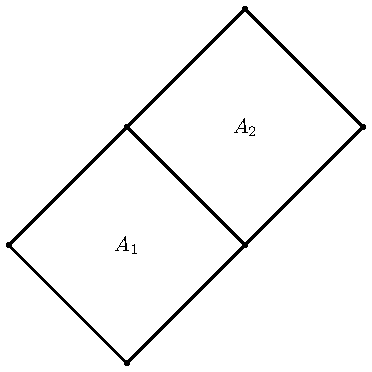
\includegraphics[width=0.85\textwidth]{figures/planar_subdivision}
            \tiny{Planar subdivision} \\
            \vspace{0.25cm}
            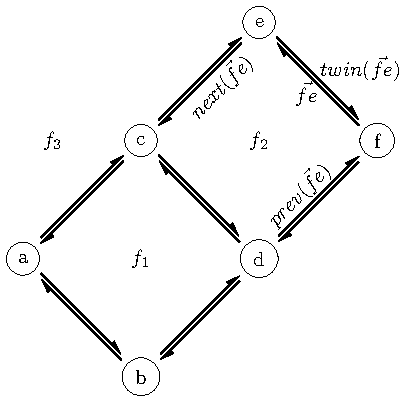
\includegraphics[width=\textwidth]{figures/dcel_representation1}
            \tiny{DCEL representation}
        \end{minipage}
    \end{frame}

    \begin{frame}{DCEL description}
        \begin{itemize}
                \item DCEL uses three tables: Vertices, Faces and Half-edges.
        \end{itemize}
        \vspace{0.25cm}
        \begin{minipage}{0.79\textwidth}
            \centering
            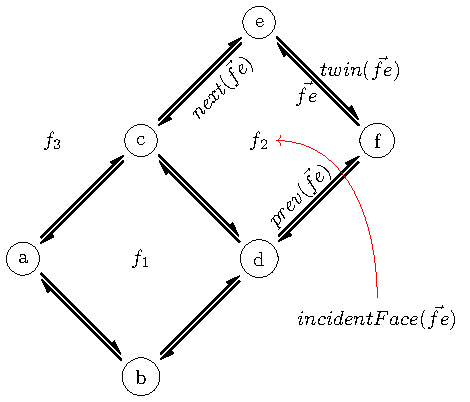
\includegraphics[width=0.8\textwidth]{figures/dcel_representation2}
        \end{minipage}\hfill % maximize the horizontal separation
    \end{frame}

   \begin{frame}{DCEL description}
        \begin{itemize}
                \item DCEL uses three tables: Vertices, Faces and Half-edges.
        \end{itemize}
        \vspace{0.25cm}
        \begin{minipage}{0.49\textwidth}
            \centering
            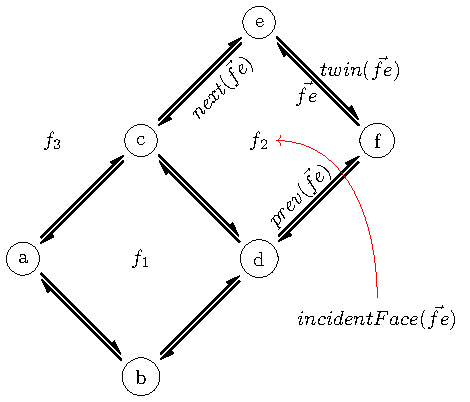
\includegraphics[width=0.85\textwidth]{figures/dcel_representation2}
        \end{minipage}\hfill % maximize the horizontal separation
        \begin{minipage}{0.49\textwidth}
            \centering

            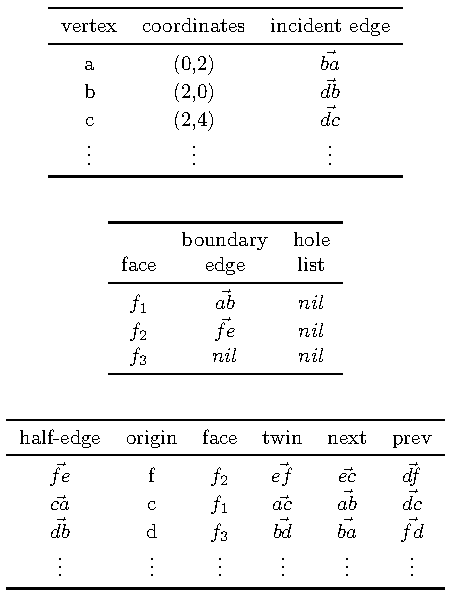
\includegraphics[width=0.85\textwidth]{figures/dcel_records}
        \end{minipage}
    \end{frame}

    \begin{frame}{DCEL Advantages}
        \begin{itemize}
            \item \textbf{Efficiency}: very efficient for computation of  \textit{overlay operators}.
            \item \textbf{Re-usability}: allows multiple operations over the same DCEL.
            \item \textbf{Pipelining}: the output of a DCEL operator can be input to another DCEL operator.
        \end{itemize}
        \vspace{0.25cm}

        \centering

        \begin{tikzpicture}
        \node (A) {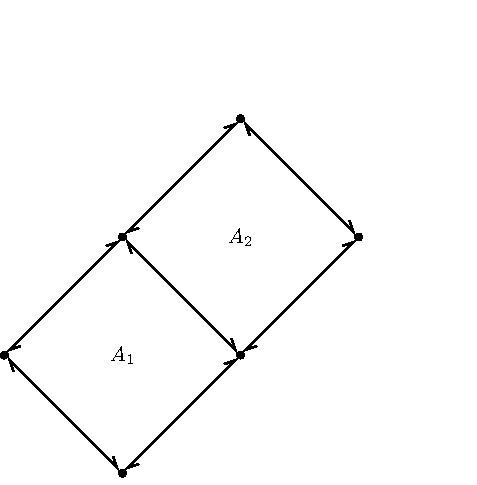
\includegraphics[width=0.4\textwidth]{figures/A}};
        \pause
        \node (X) {
\includegraphics[width=0.5\textwidth]{figures/blank}};
        \node (B) {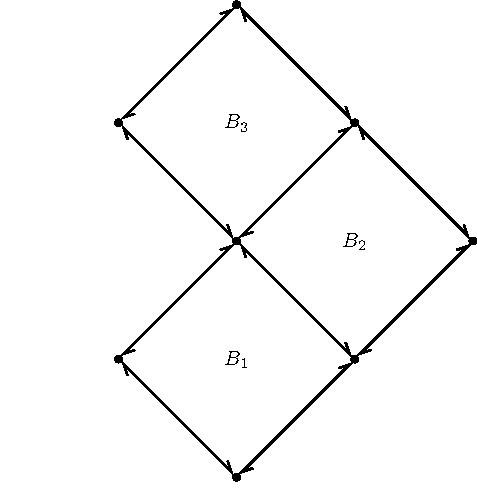
\includegraphics[width=0.4\textwidth]{figures/B}};
        \pause
        \node (X) {
\includegraphics[width=0.5\textwidth]{figures/blank}};
        \node (AB) {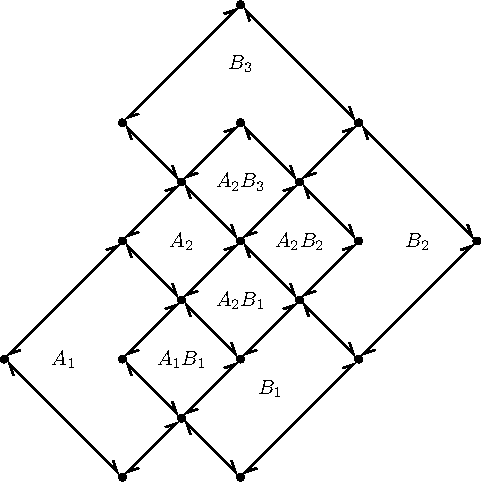
\includegraphics[width=0.4\textwidth]{figures/AB}};
        \pause
        \node (X) {
\includegraphics[width=0.5\textwidth]{figures/blank}};
        \node (O) {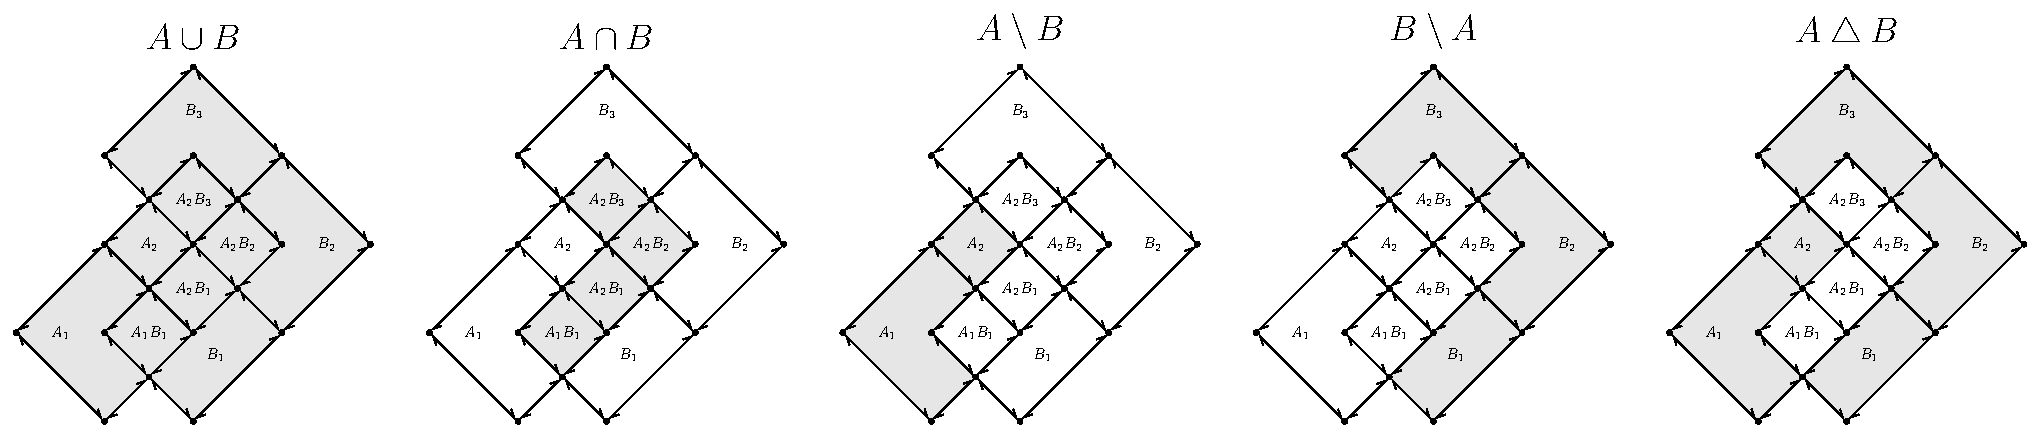
\includegraphics[width=\textwidth]{figures/dcel_operators}};
        \end{tikzpicture}

    \end{frame}

    \begin{frame}{Challenges and Contributions}
        \begin{itemize}
            \item Currently only sequential DCEL implementations exist.
            \item Unable to deal with large datasets (i.e. US Census tracks at national level).
            \item We propose a \textit{scalable} \textit{distributed} approach to compute the overlay of two polygon layers using DCELs.
            \item Distribution enables scalability, but introduces challenges: the \textbf{\textit{orphan-cell}} problem and the \textbf{\textit{orphan-hole}} problem.
        \end{itemize}

    \end{frame}

    \begin{frame}{Sequential implementation}
        \begin{itemize}
                \item Consider two (simple) input DCELs $A_1$ and $B_1$.  The sequential algorithm first finds the intersections of half-edges.
                \item Then, new vertices (e.g. $c_1, c_2$) are created,  half-edges are updated, new faces are added and labeled (e.g. $A_1B_1$).
        \end{itemize}
        \vspace{0.5cm}

        \centering
        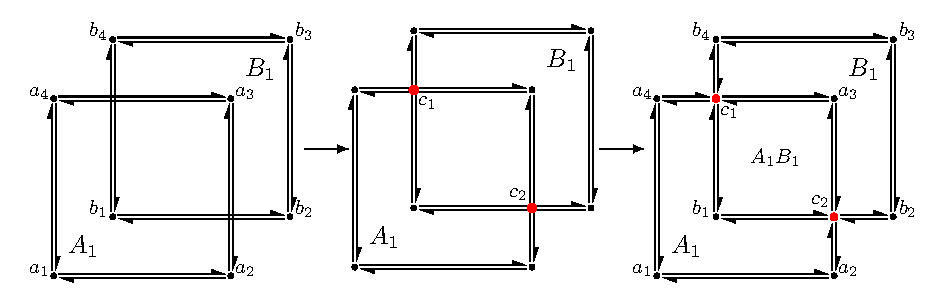
\includegraphics[width=\textwidth]{../thesis/chapterSDCEL/dcel2}
    \end{frame}

    \begin{frame}{Scalable Implementation}
        \begin{itemize}
            \small
            \item Two phases: (1) Distributed DCEL construction, and (2) Distributed overlay evaluation.
            \item Distribution is based on a spatial index (e.g. quadtree)
            \item Each input DCEL layer (e.g. A, B) is partitioned using the same index
        \end{itemize}
        \vspace{0.25cm}

        \centering
        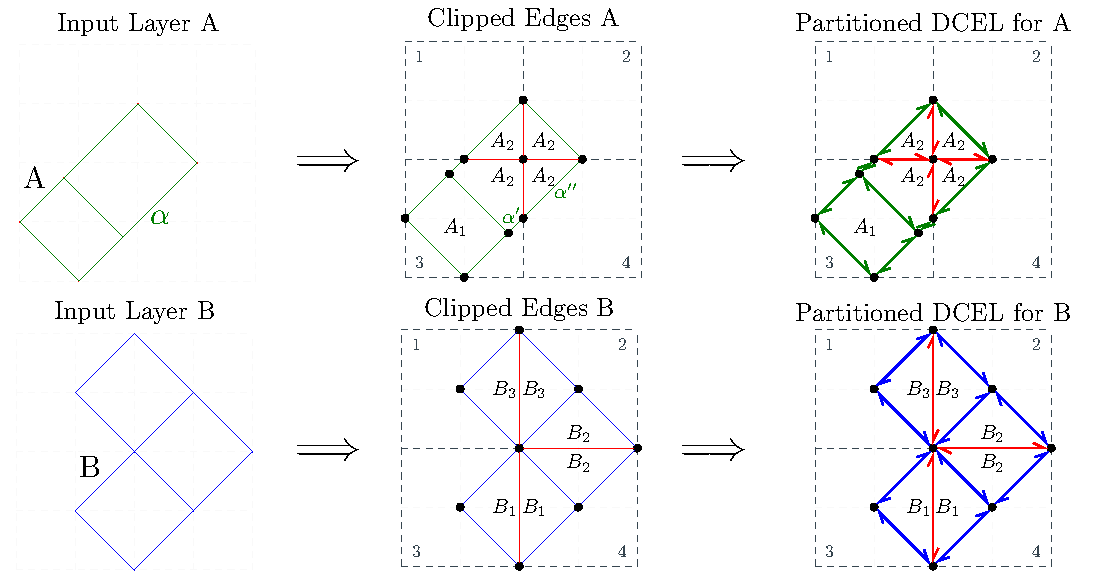
\includegraphics[width=0.8\textwidth]{../thesis/chapterSDCEL/partition_schema/PolygonsParted}
    \end{frame}

    \begin{frame}{Scalable Implementation}
        \begin{itemize}
            \small
            \item Each index cell should contain all information needed so that it can compute the overlay DCEL locally
            \item For each cell to be independent, we need to create "artificial" edges and vertices
        \end{itemize}
        \vspace{0.25cm}

        \centering
        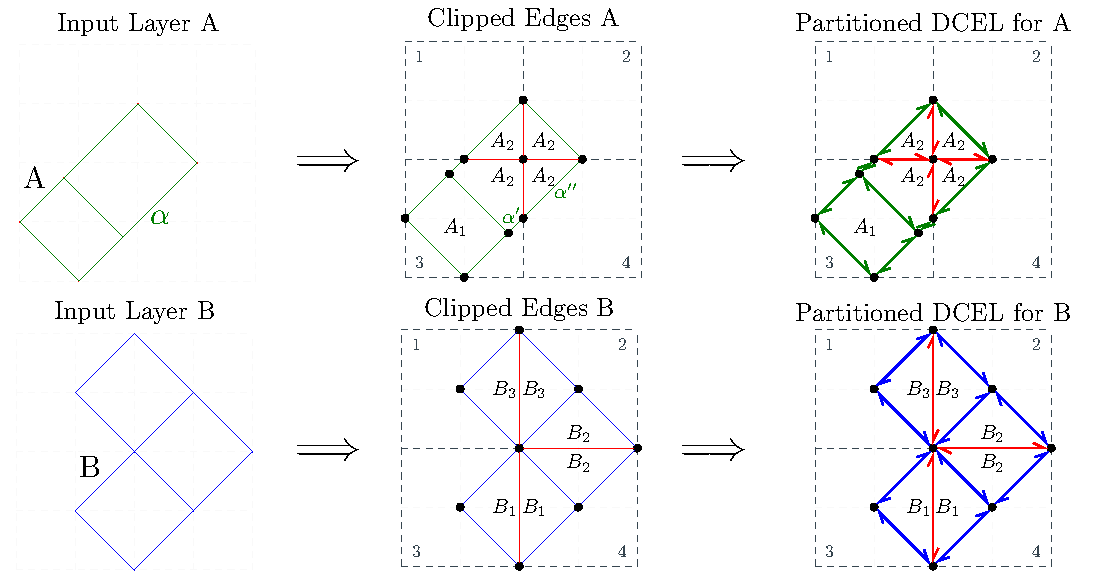
\includegraphics[width=0.8\textwidth]{../thesis/chapterSDCEL/partition_schema/PolygonsParted}
    \end{frame}

    \begin{frame}{Distributed DCEL construction}
        \centering
        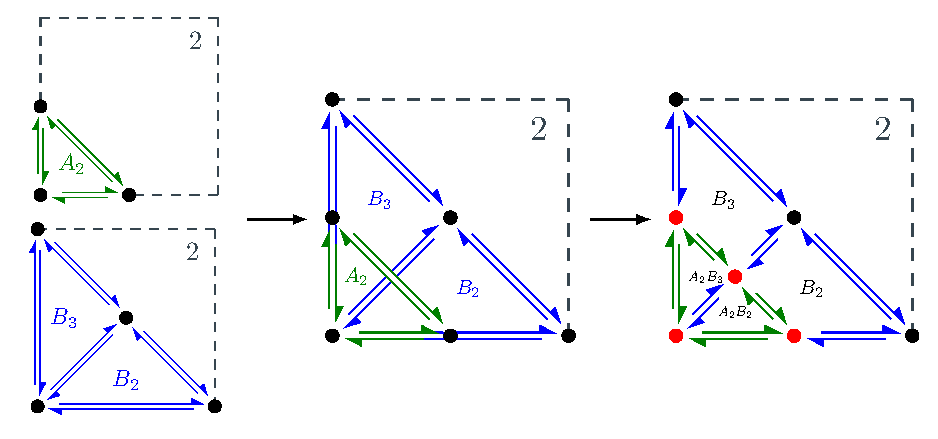
\includegraphics[width=0.65\textwidth]{../thesis/chapterSDCEL/overlay_partition/overlay_partition} \\
        \vspace{0.5cm}
        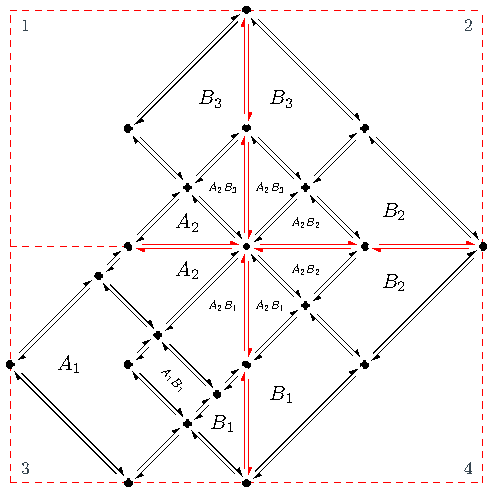
\includegraphics[width=0.35\textwidth]{../thesis/chapterSDCEL/distributed_dcel}
    \end{frame}

   \begin{frame}{Overlay evaluation}
        \begin{itemize}
            \item Answering global overlay queries...
            \begin{itemize}
                \item To compute a particular overlay operator, we query local DCELs.
                \item This work is done independently at each cell (node).
                \item SDCEL then collects back all local DCEL answers and computes the final answer (by removing artificial edges and concatenating the resulting faces).
            \end{itemize}
        \end{itemize}
        \vspace{0.5cm}

        \centering
        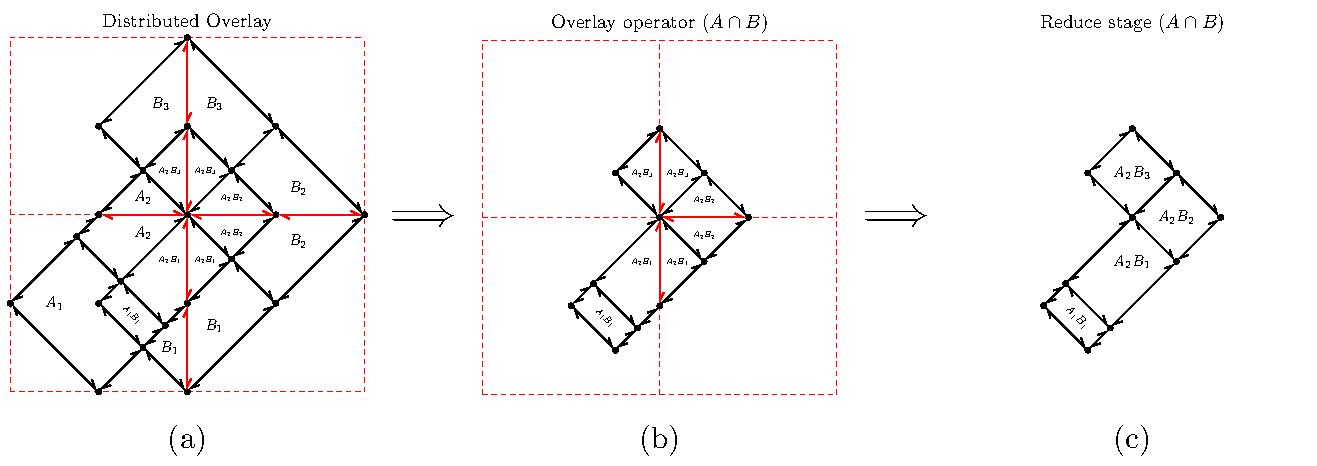
\includegraphics[width=\textwidth]{../thesis/chapterSDCEL/overlay_operator}
    \end{frame}


    \begin{frame}{Labeling orphan cells and orphan holes}
        \begin{minipage}{0.59\textwidth}
            \begin{itemize}
                \item We next discuss the \textbf{orphan cell} problem (orphan holes are handled similarly).
                \item A large face (e.g. the red polygon in the figure) can contain cells that do not intersect with any of the face's boundary edges (called \textit{regular edges}).
                \item Such cells do not contain any label and thus we do not know which face they belong to.
            \end{itemize}
        \end{minipage}\hfill % maximize the horizontal separation
        \begin{minipage}{0.4\textwidth}
            \centering
            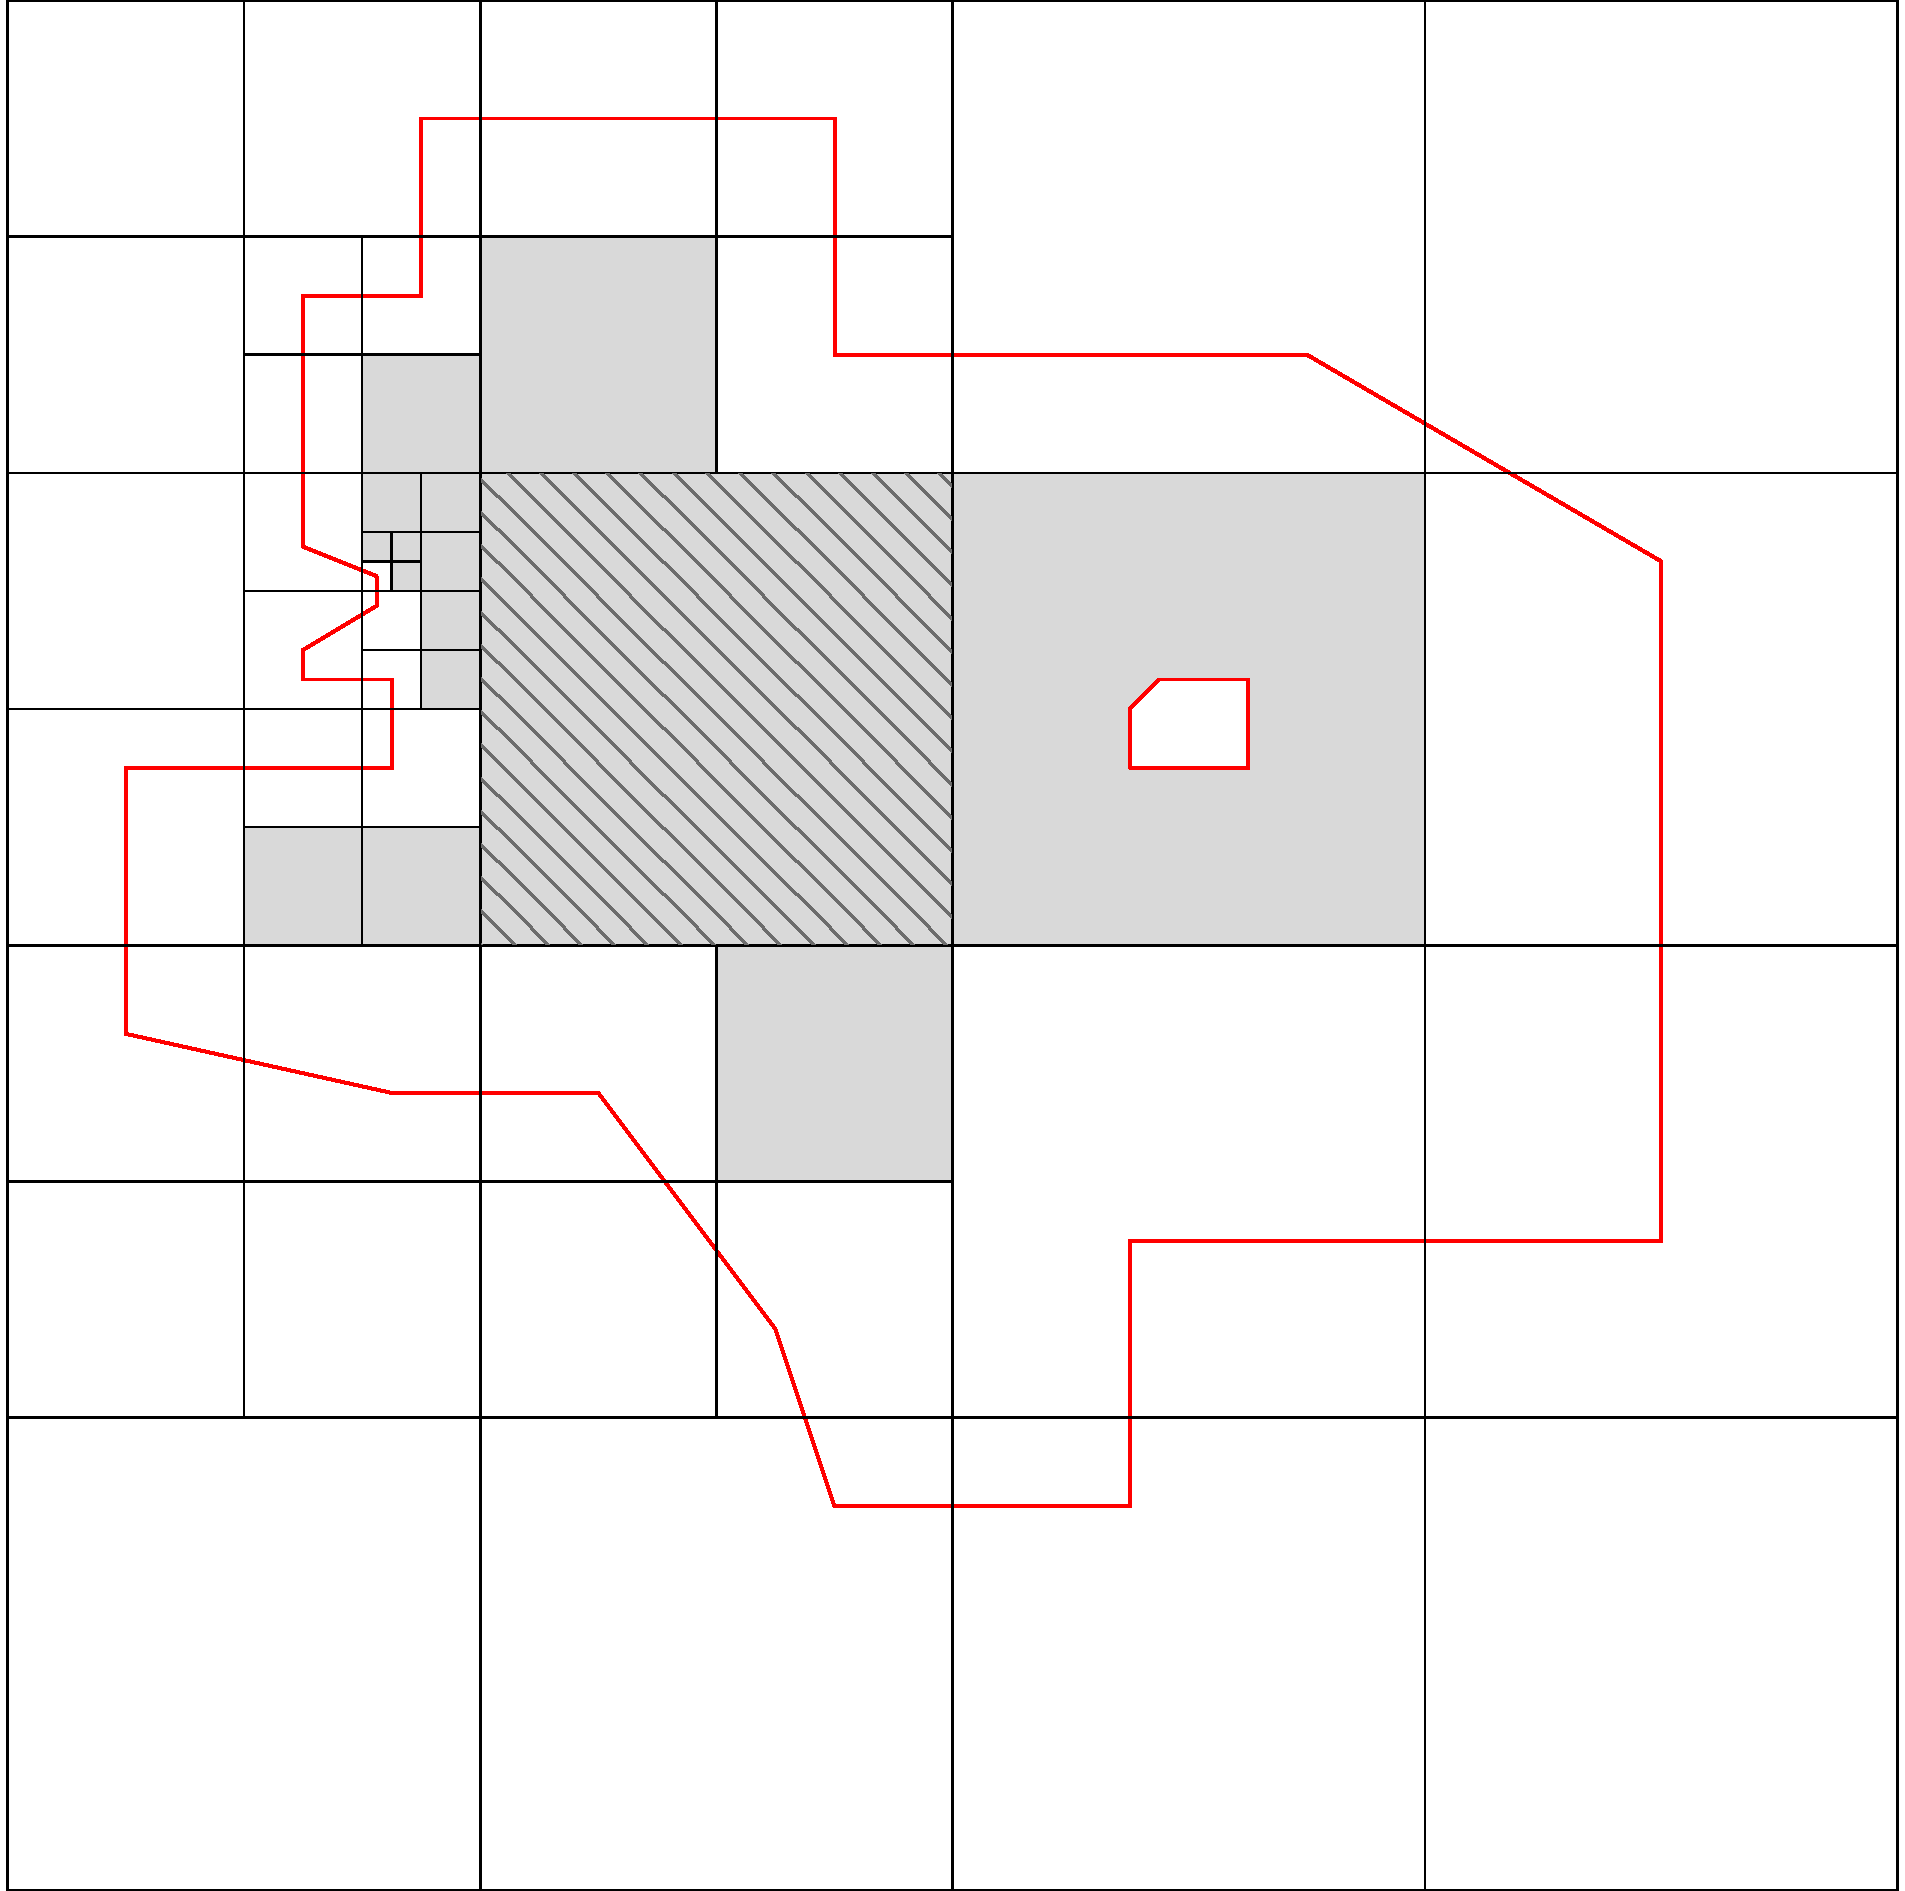
\includegraphics[width=\textwidth]{../thesis/chapterSDCEL/orphan_cells/emptycells}
            \end{minipage}
    \end{frame}

    \begin{frame}{Labeling orphan cells and orphan holes}
        \begin{itemize}
            \item We provide an algorithm to efficiently solve the orphan cell problem.
        \end{itemize}
        \vspace{0.25cm}

        \centering

        \begin{tikzpicture}
        \node (A) {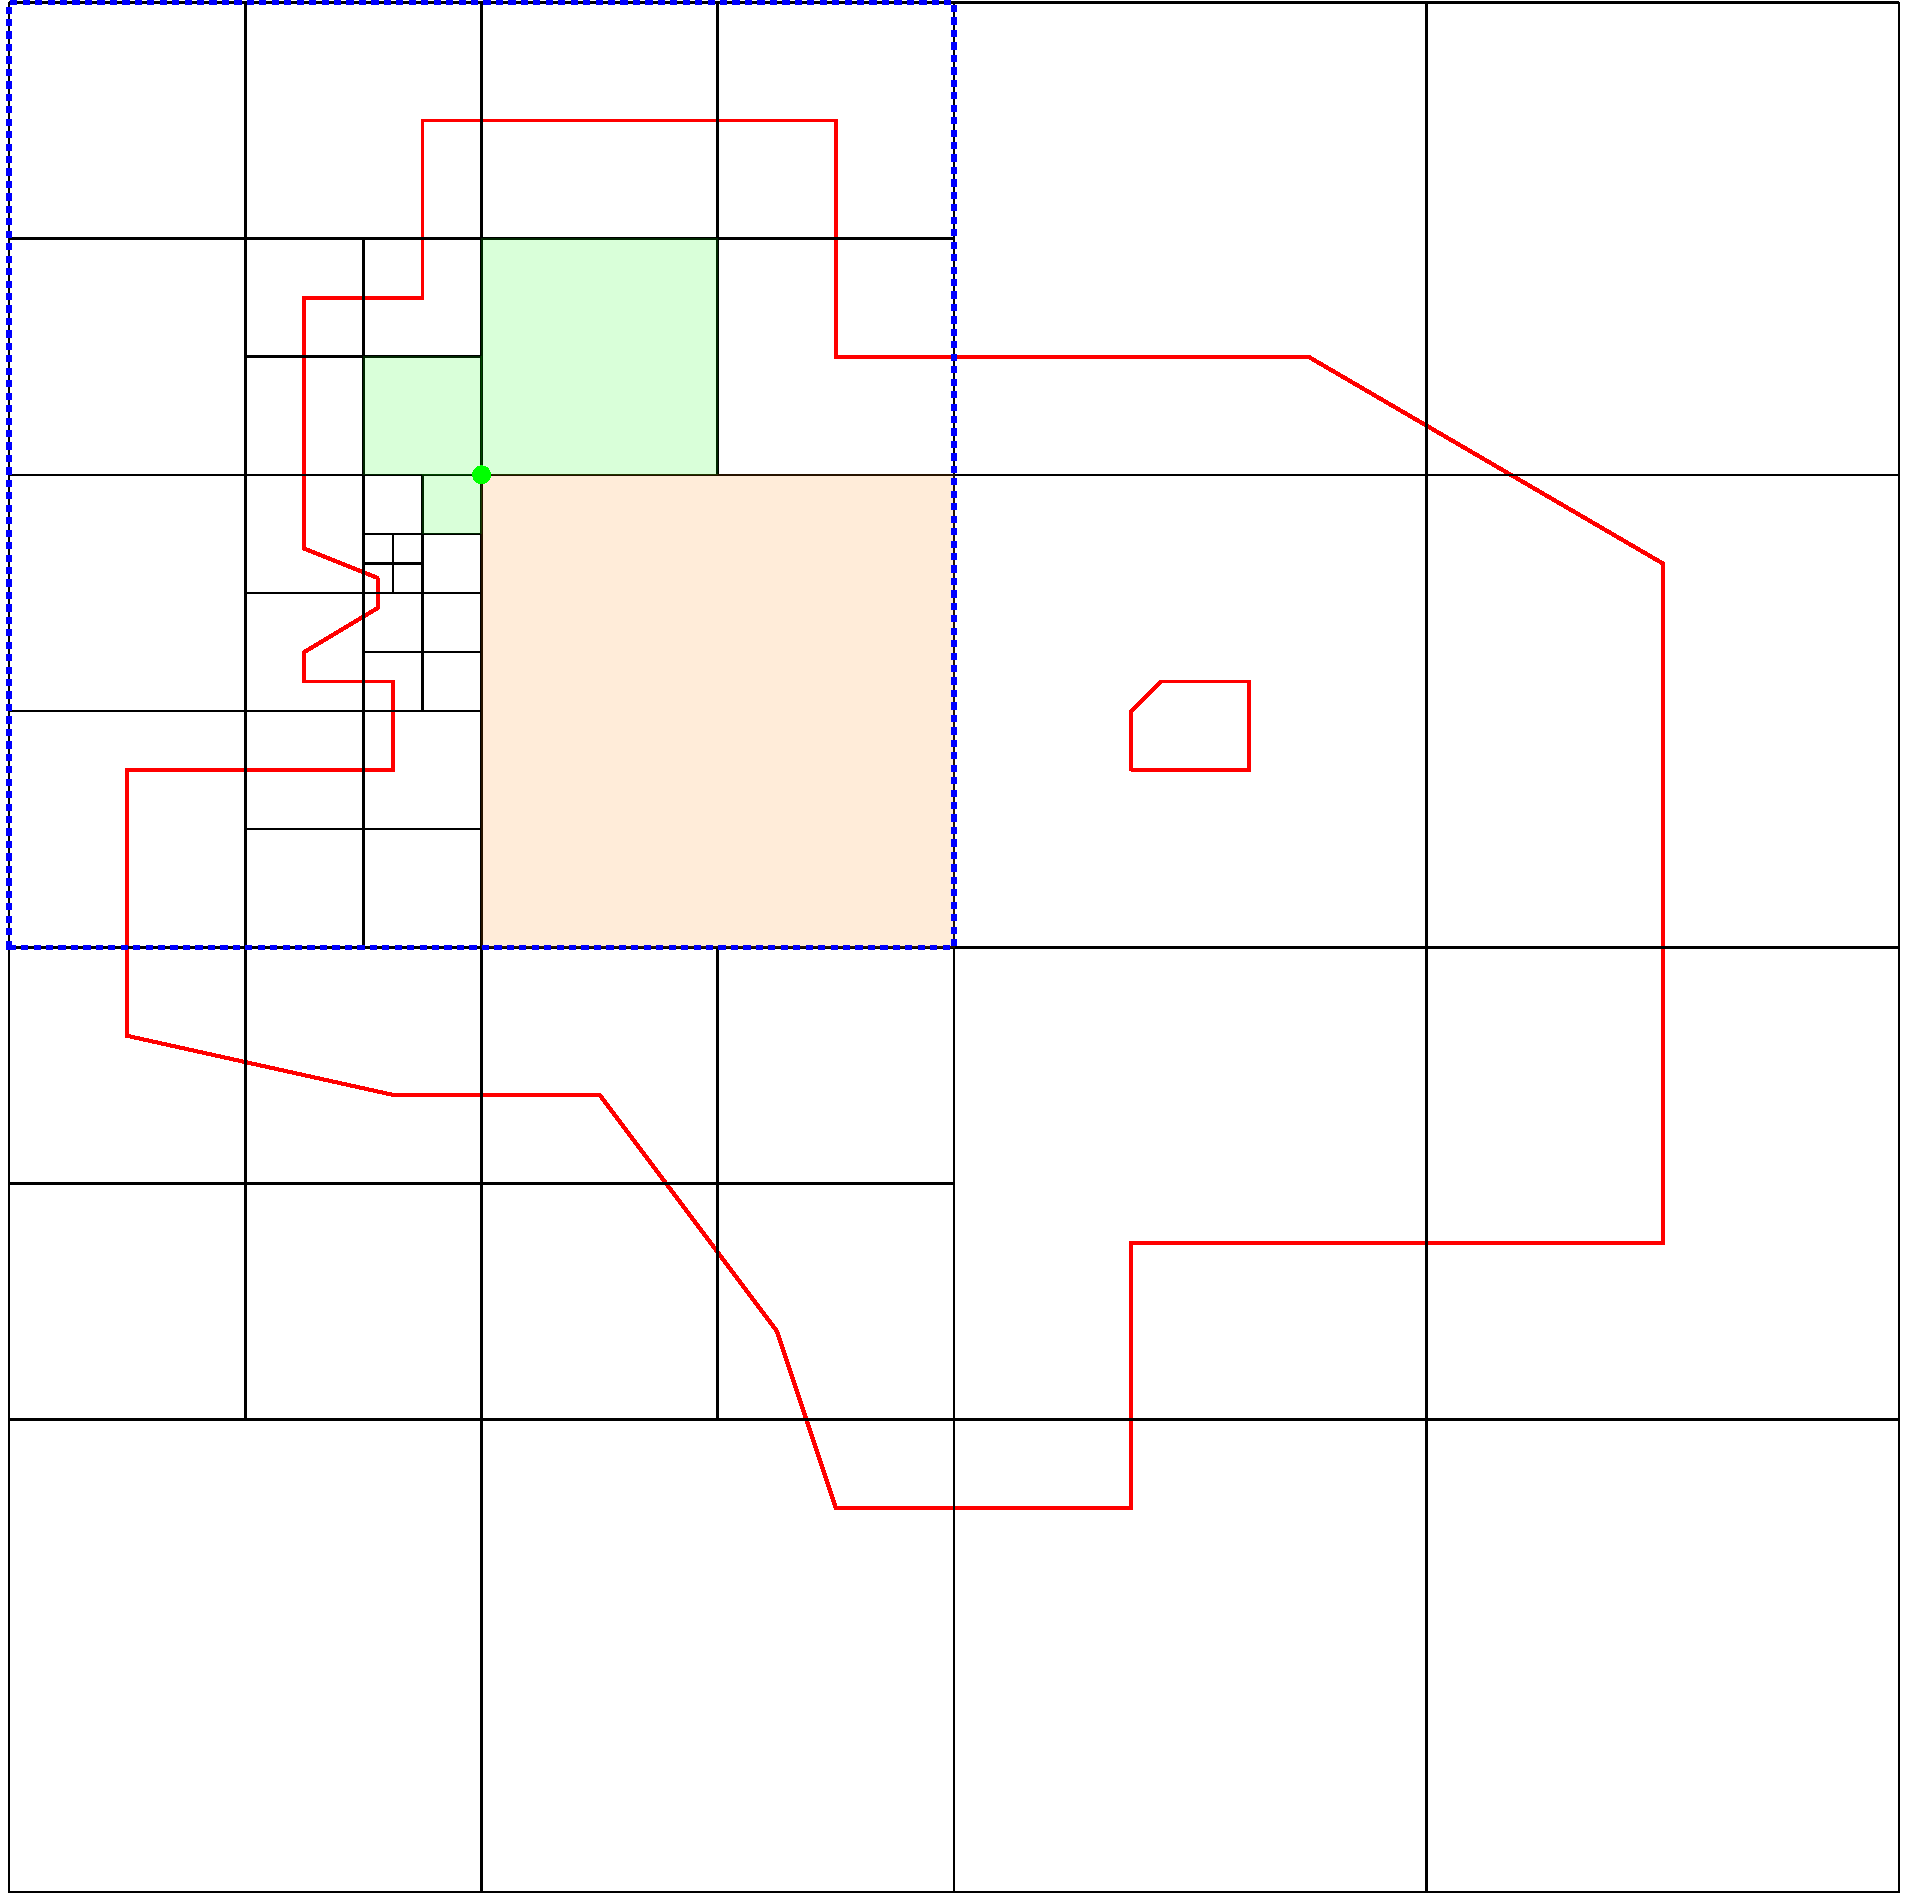
\includegraphics[width=0.5\textwidth]{../thesis/chapterSDCEL/orphan_cells/example1}};
        \pause
        \node (X) {
\includegraphics[width=0.6\textwidth]{figures/blank}};
        \node (B) {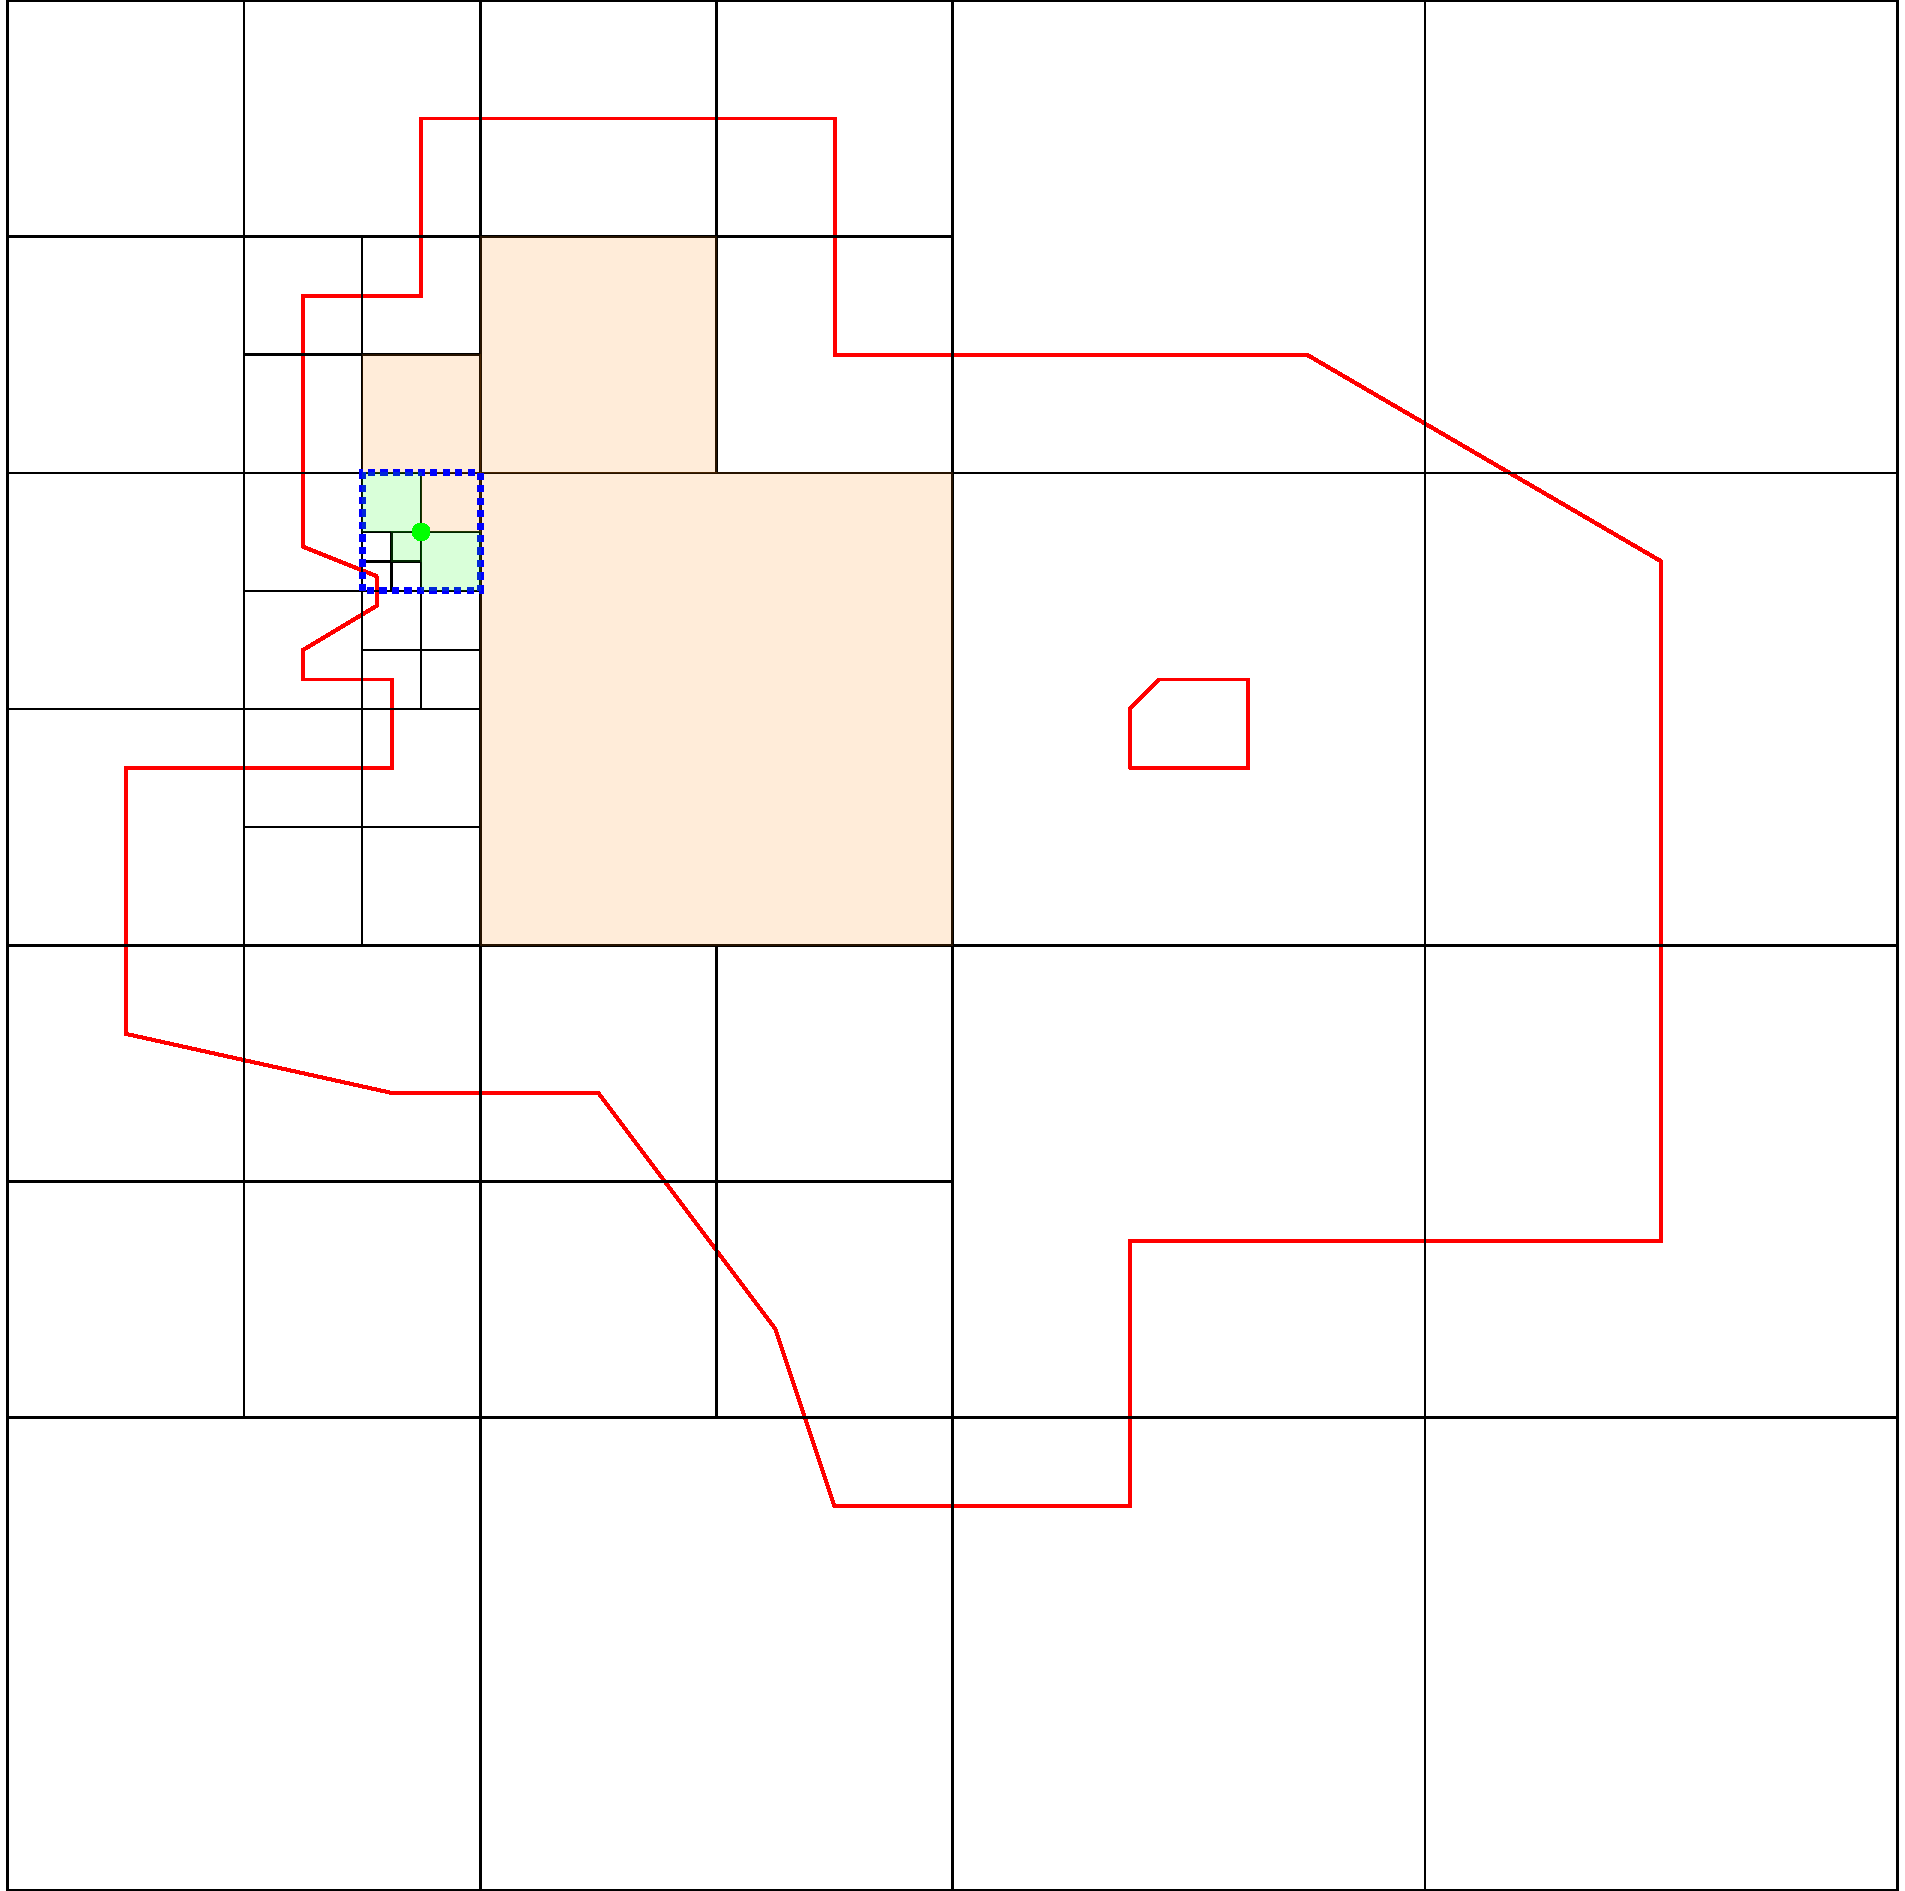
\includegraphics[width=0.5\textwidth]{../thesis/chapterSDCEL/orphan_cells/example2}};
        \pause
        \node (X) {
\includegraphics[width=0.6\textwidth]{figures/blank}};
        \node (C) {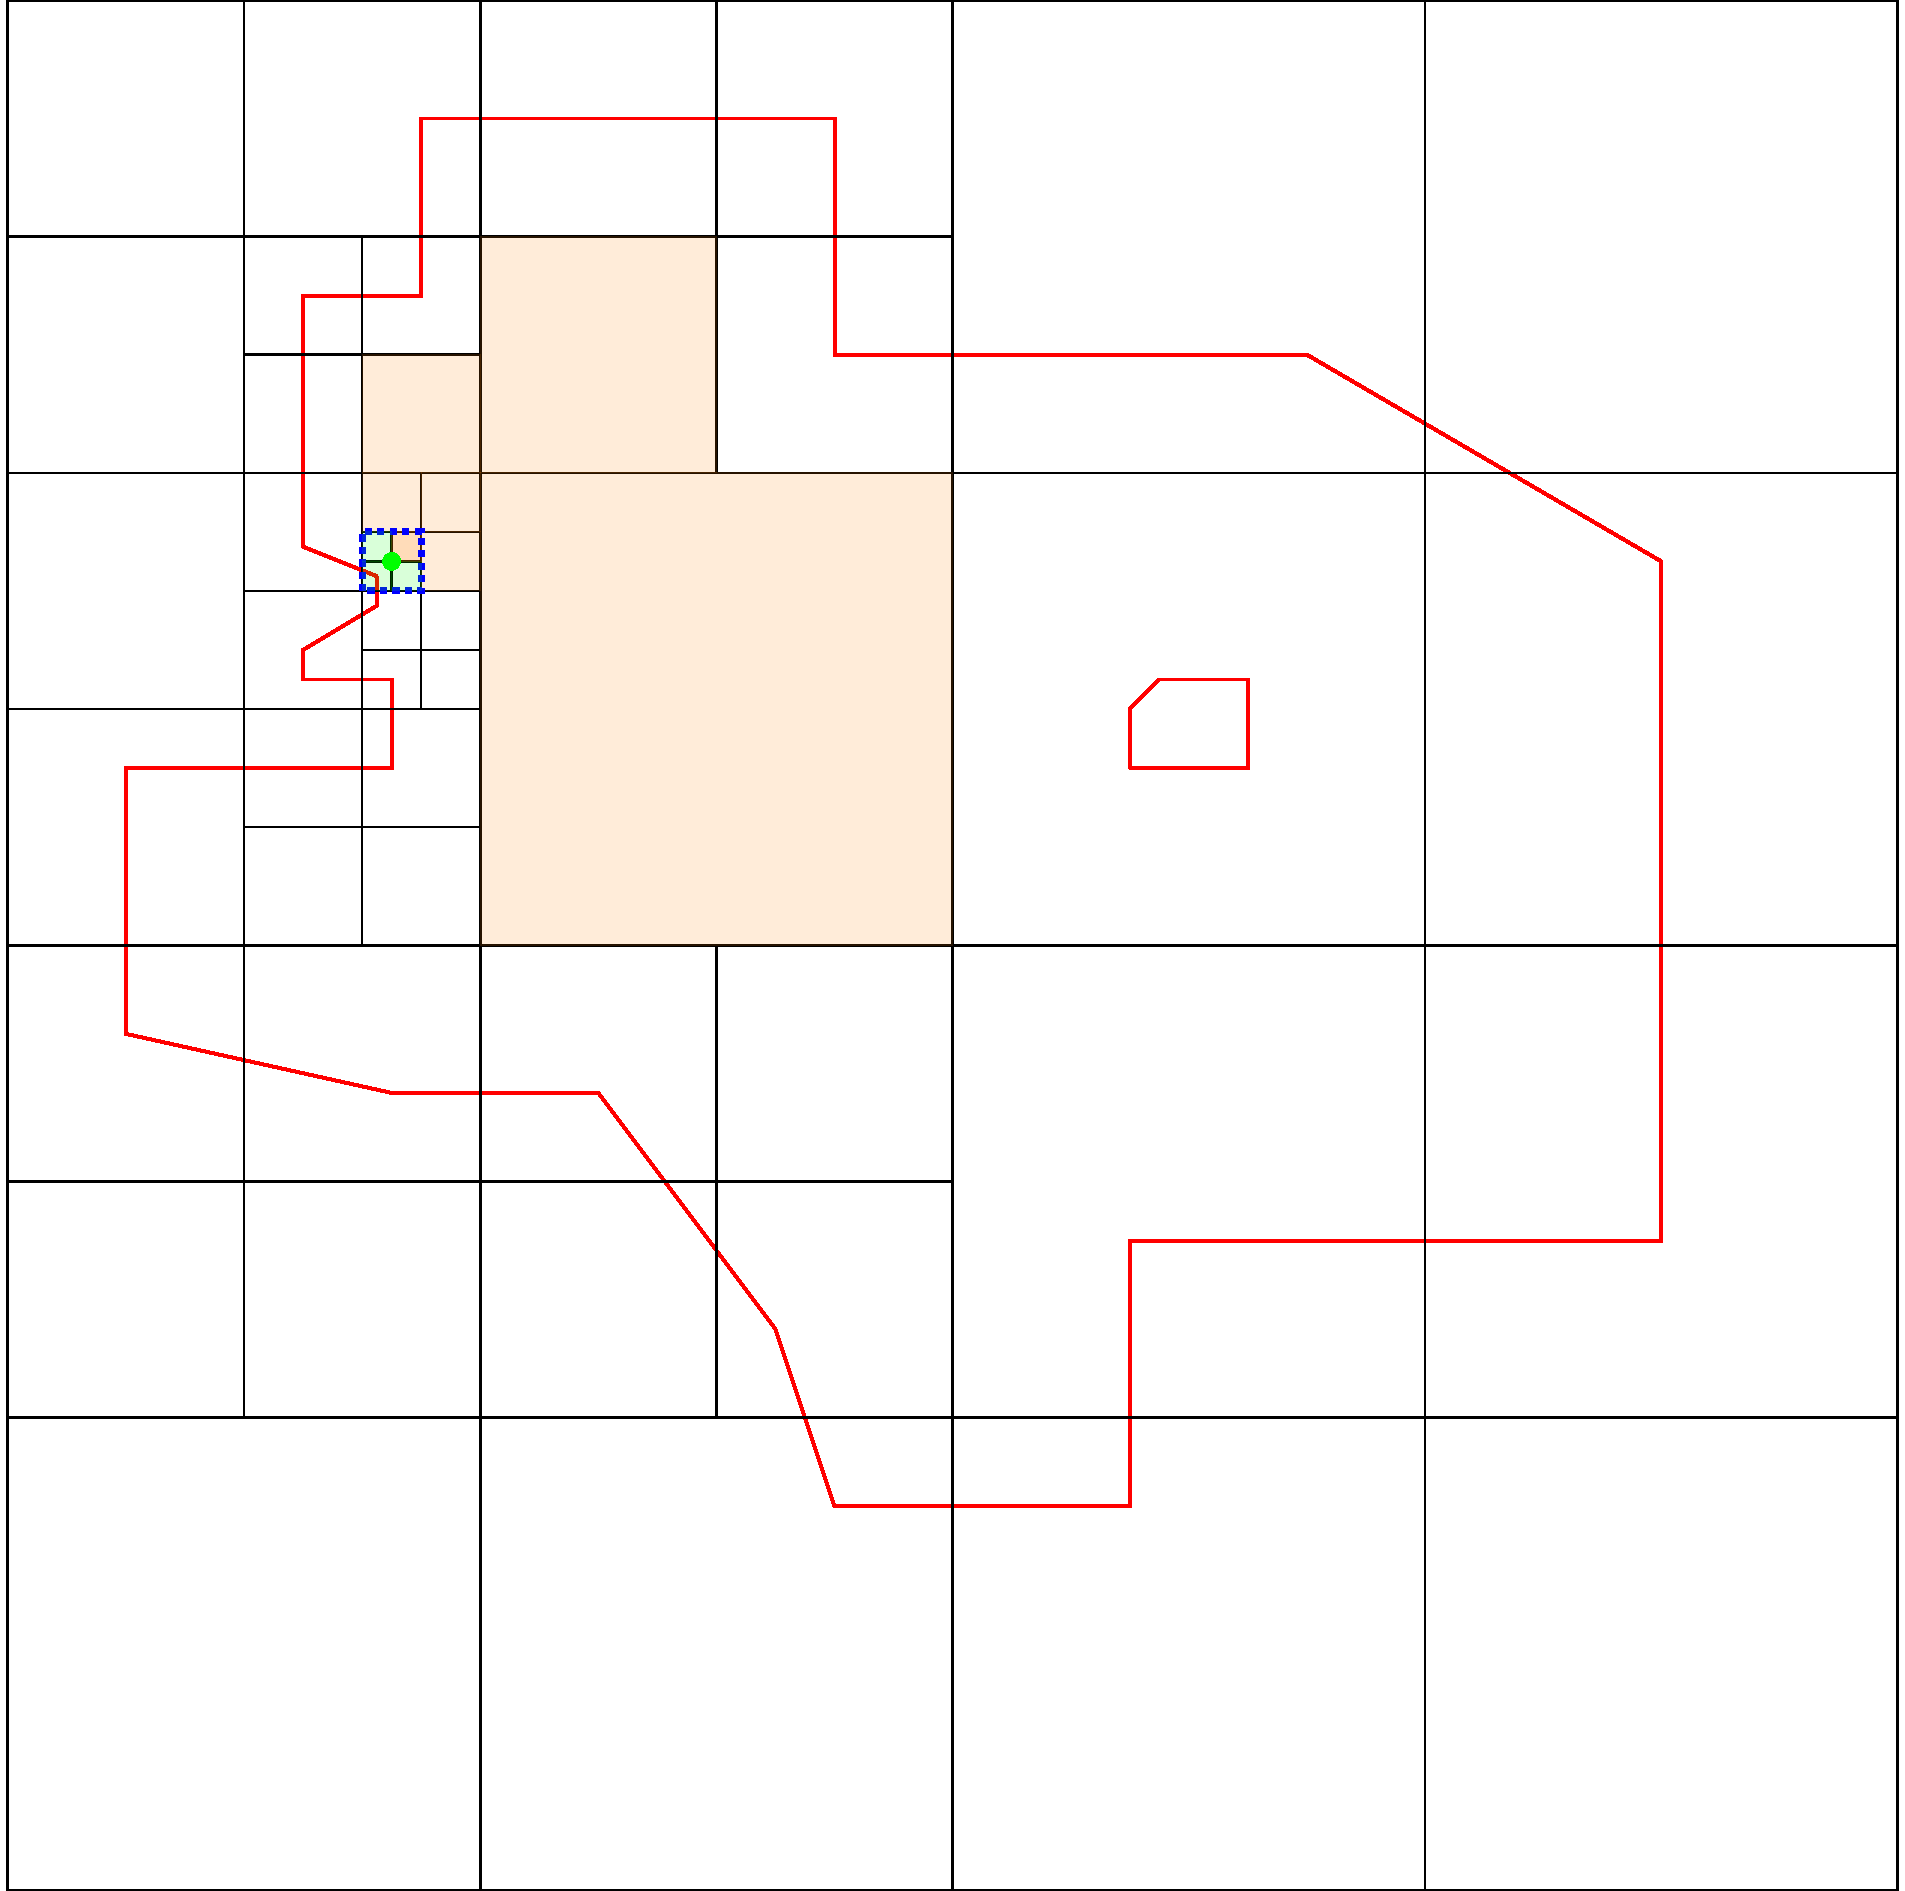
\includegraphics[width=0.5\textwidth]{../thesis/chapterSDCEL/orphan_cells/example3}};
        \end{tikzpicture}

    \end{frame}

    \begin{frame}{Overlay optimizations}
        \begin{itemize}
            \item Optimizing for faces overlapping many cells...
                \begin{itemize}
                    \item Naive approach sends all faces that overlap a cell to a master node (that will combine them).
                    \item We propose an intermediate reduce processing step.
                    \begin{itemize}
                    \item The user provides a level in the quadtree structure and faces are evaluated at those intermediate reducers.
                   \end{itemize}
                   \item We also consider another approach that re-partitions such faces using their labels as the key.
                    \begin{itemize}
                    \item It avoids the reduce phase but implies an additional shuffle.
                    \item However, as we show in the experiments this overhead is minimal.
                    \end{itemize}
                \end{itemize}
        \end{itemize}
    \end{frame}

    \begin{frame}{Overlay optimizations}
        \begin{itemize}
            \item Optimizing for unbalanced layers...
                \begin{itemize}
                    \item Finding intersections is the most critical part of the overlay computation.
                    \item However, in many cases one of the layers has much more half-edges than the other.
                    \item Sweep-line algorithms to detect intersections run over all the edges.
                    \item Instead we scan the larger dataset only for the x-intervals where there are half-edges from the smaller dataset.
                \end{itemize}
        \end{itemize}
    \end{frame}

    \begin{frame}{Experimental evaluation}
        \begin{itemize}
            \item Datasets.
        \end{itemize}
        \vspace{1cm}
        \centering
        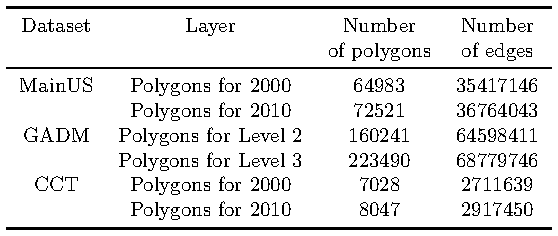
\includegraphics[width=0.9\textwidth]{figures/sdcel_datasets}
    \end{frame}

    \begin{frame}{Experimental evaluation}
        \begin{itemize}
            \item Evaluation of the overlapping faces optimization.
        \end{itemize}
        \vspace{5mm}
        \centering
        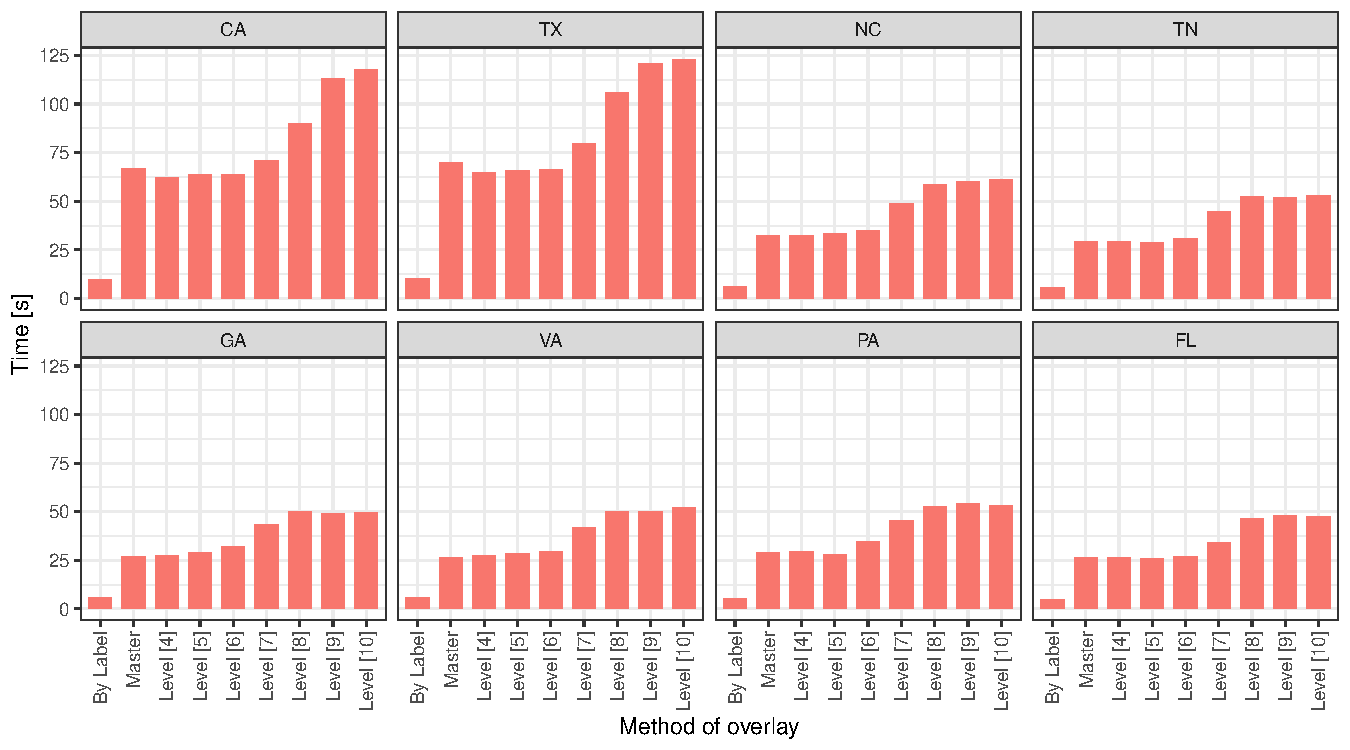
\includegraphics[width=0.9\textwidth]{../thesis/chapterSDCEL/OverlayTester/Overlay_Tester}
    \end{frame}

    \begin{frame}{Experimental evaluation}
        \begin{itemize}
            \item Evaluation of the unbalanced layers optimization.
        \end{itemize}
        \vspace{5mm}
        \centering
        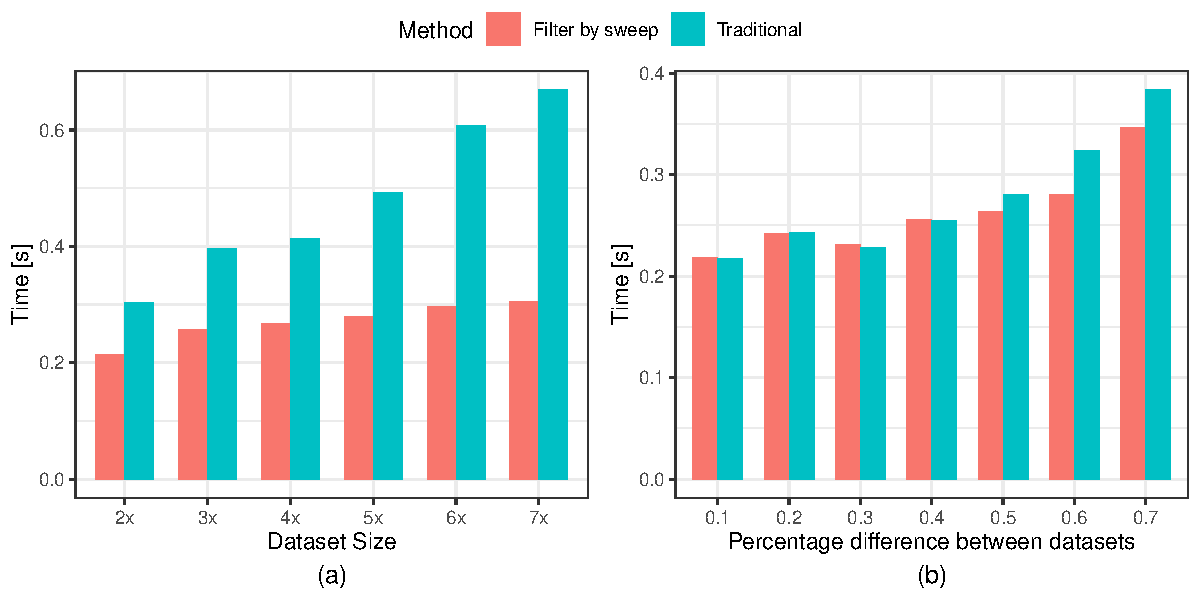
\includegraphics[width=\textwidth]{../thesis/chapterSDCEL/UnbalanceTester/Unbalance_Tester}
    \end{frame}

    \begin{frame}{Experimental evaluation}
        \begin{itemize}
            \item Performance varying number of partition cells (CCT dataset).
        \end{itemize}
        \vspace{1cm}

        \begin{minipage}{0.49\textwidth}
            \centering
            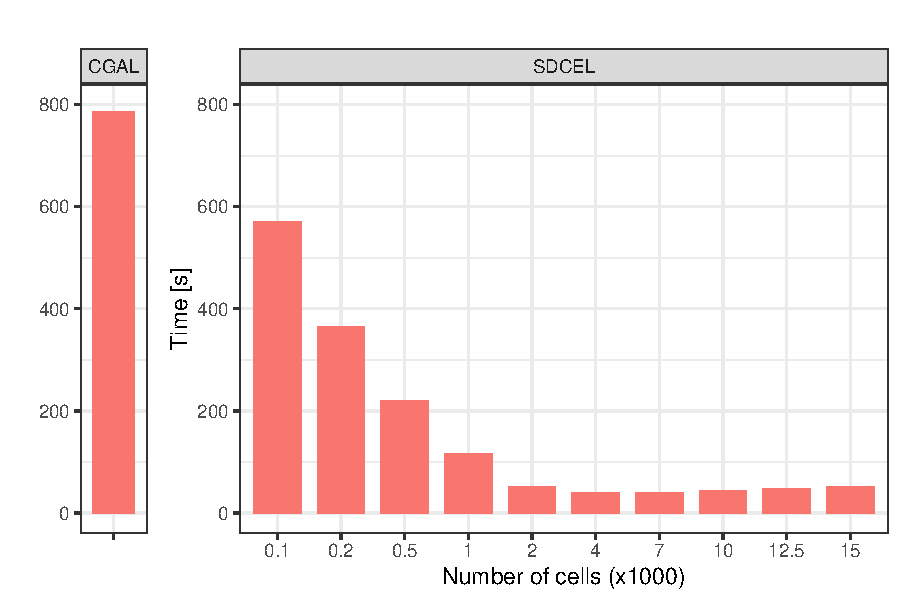
\includegraphics[width=\textwidth]{../thesis/chapterSDCEL/CA/CA}
        \end{minipage}\hfill % maximize the horizontal separation
        \begin{minipage}{0.49\textwidth}
            \centering
            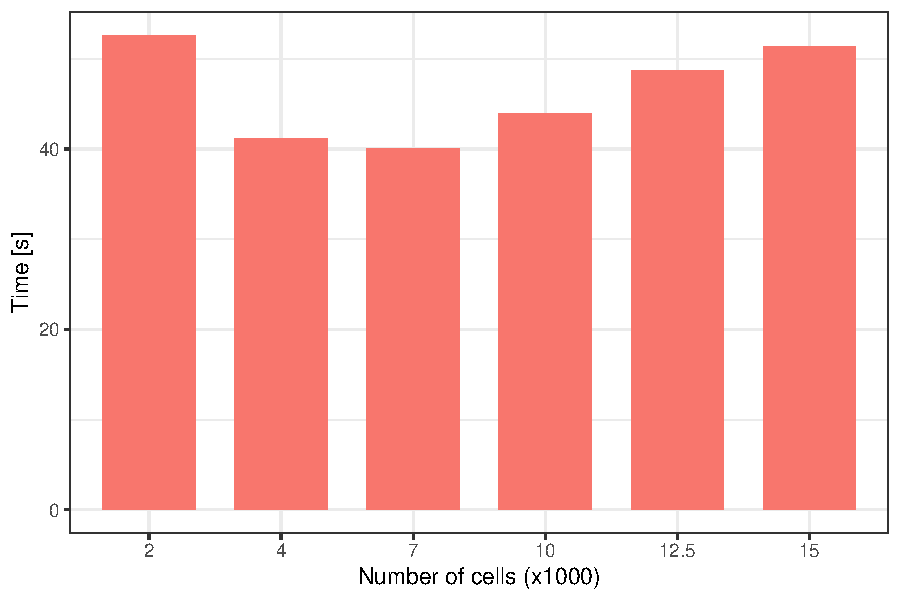
\includegraphics[width=0.95\textwidth]{../thesis/chapterSDCEL/CA/CA_sample}
        \end{minipage}
    \end{frame}

    \begin{frame}{Experimental evaluation}
        \begin{itemize}
            \item Performance with MainUS and GADM datasets.
        \end{itemize}
        \vspace{5mm}
        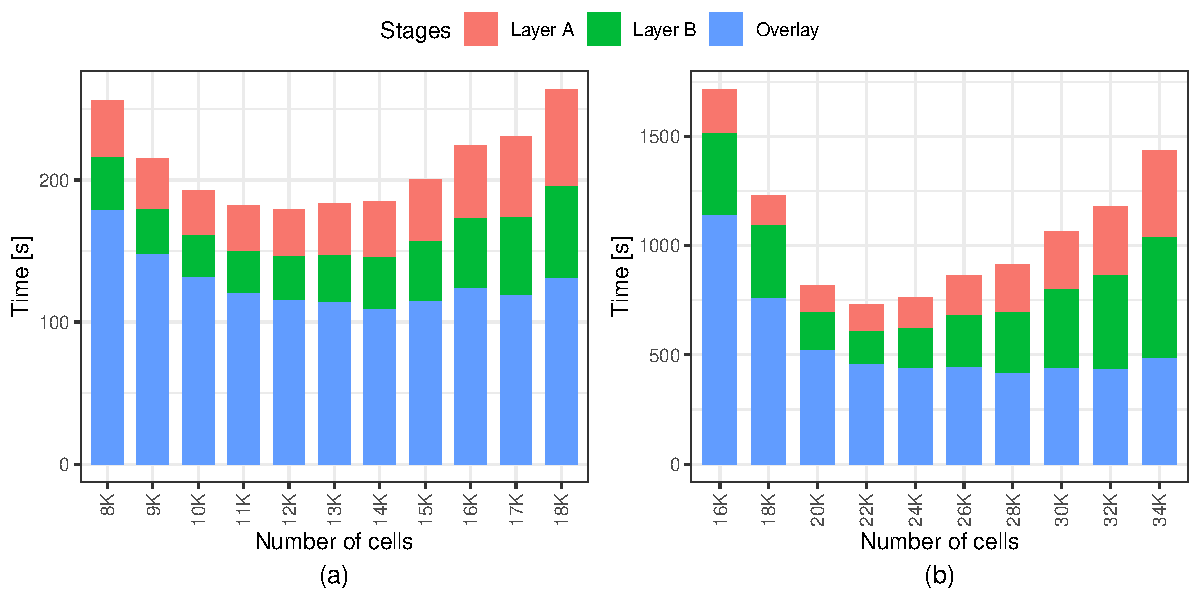
\includegraphics[width=\textwidth]{../thesis/chapterSDCEL/Performance/Performance}
    \end{frame}

    \begin{frame}{Experimental evaluation}
        \begin{itemize}
            \item MainUS scale-up and speed-up.
        \end{itemize}
        \vspace{5mm}
        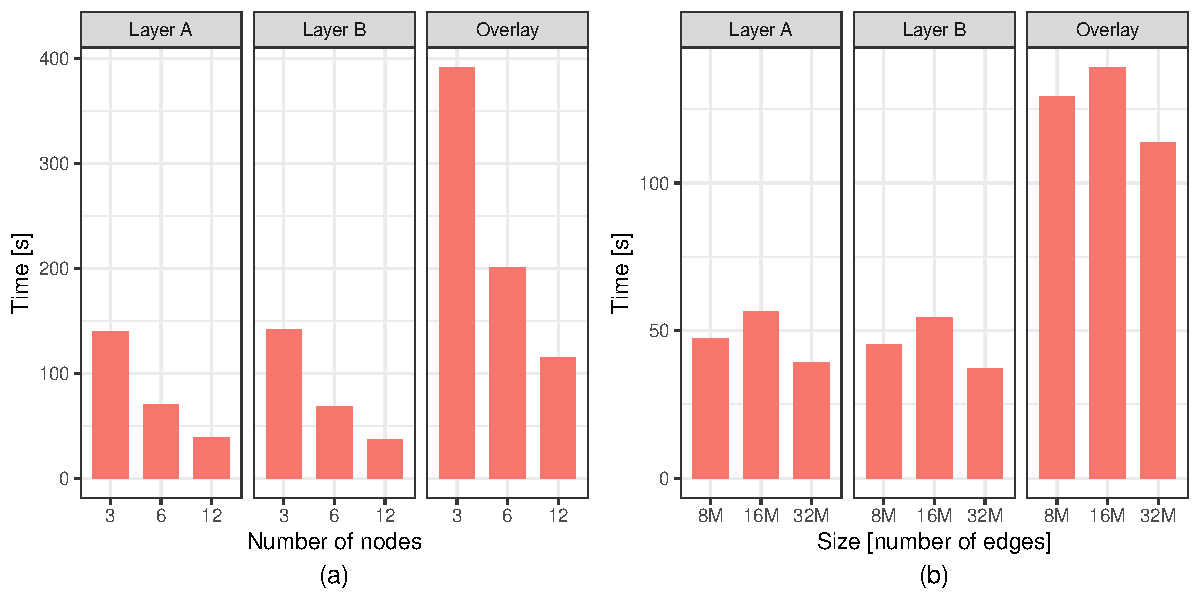
\includegraphics[width=\textwidth]{../thesis/chapterSDCEL/MainUS_SS/MainUS_SS}
    \end{frame}

    \begin{frame}{Experimental evaluation}
        \begin{itemize}
            \item GADM scale-up and speed-up.
        \end{itemize}
        \vspace{5mm}
        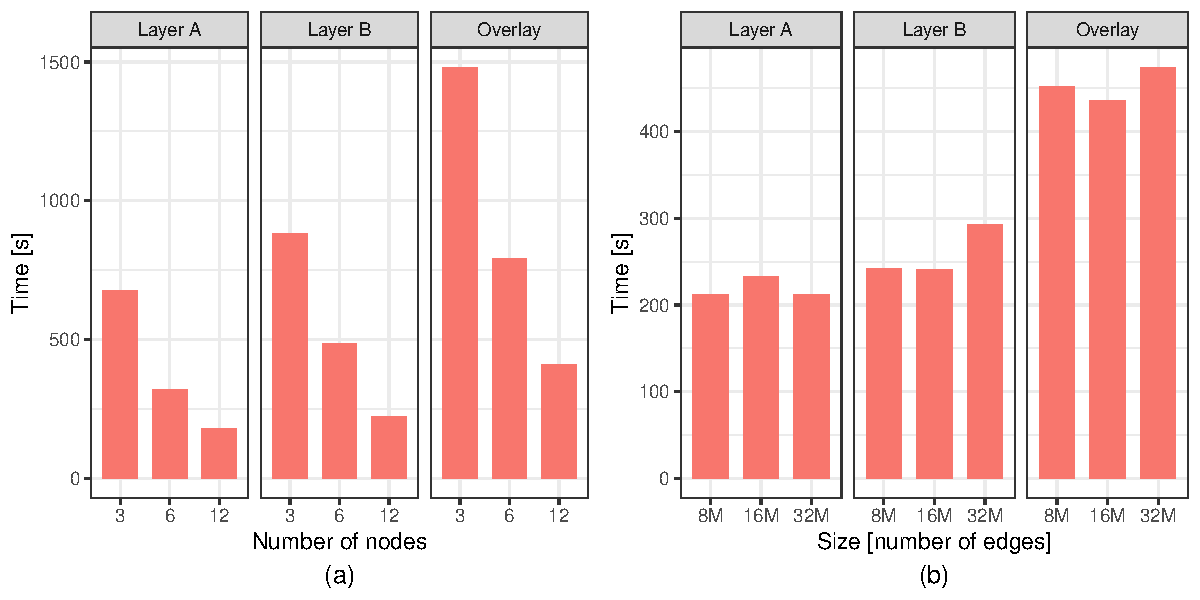
\includegraphics[width=\textwidth]{../thesis/chapterSDCEL/GADM_SS/GADM_SS}
    \end{frame}

%     \begin{frame}{Conclusions}
%         \begin{itemize}
%             \item We introduced SDCEL, a scalable approach to compute the overlay operation among two layers that represent polygons from a planar subdivision of a surface.
%             \item We use a partition strategy which guarantees that each partition (cell) has the data needed to work independently.
%             \item We also proposed several optimizations to improve performance.
%             \item Our experiments using real datasets show very good performance; we are able to compute overlays over very large layers (each with >35M edges) in few minutes.
%         \end{itemize}
%     \end{frame}

    %%%%%%%%%%%%%%%%%%%%%%%%%%%%%%%%%%%%%%%%%%%%%%
    %%%%%%%%%%%%%%%%%%%%%%%%%%%%%%%%%%%%%%%%%%%%%%

%     \begin{frame}{Outline}
%         \begin{itemize}
%                 \item Scalable overlay operations over DCEL polygons layers
%                 \item \textbf{Towards parallel detection of movement patterns in large trajectory databases}
%         \end{itemize}
%     \end{frame}

    %\section{Scalable Processing of Moving Flock Patterns}
    \begin{frame}{Large trajectory databases}
        \begin{minipage}{0.59\textwidth}
            \begin{itemize}
                \item A spatial trajectory is a trace in time generated by a moving entity in a geographical space.
                \item i.e. $p_1 \rightarrow p_2 \rightarrow \cdots \rightarrow p_n$
                \item A trajectory is stored as a set of points, $p_i = (x, y, t)$ (spatial coordinate + time stamp).
            \end{itemize}
        \end{minipage}\hfill % maximize the horizontal separation
        \begin{minipage}{0.4\textwidth}
            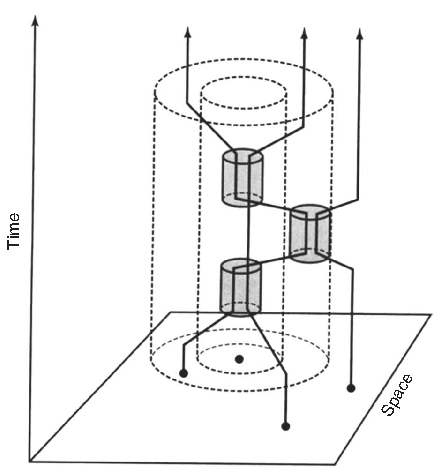
\includegraphics[width=\textwidth]{figures/trajectory}
            \begin{flushright}
                {\tiny (Shoval, 2017)}
            \end{flushright}
        \end{minipage}
    \end{frame}

    \begin{frame}{Movement patterns}
        \centering
        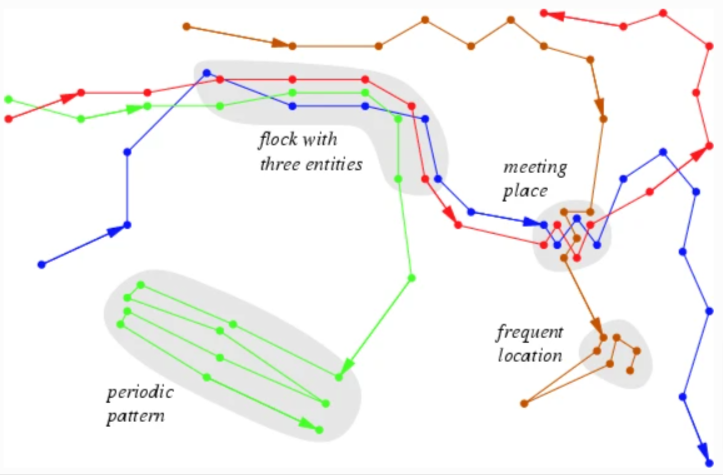
\includegraphics[width=0.55\textwidth]{figures/patterns}
        \begin{flushright}
            {\tiny (Gudmundsson, et al. 2008)}
        \end{flushright}


        \begin{itemize} \item i.e. convoys, moving clusters, swarms, gatherings, \textbf{flocks}, ... \end{itemize} \vspace{0.5cm}
    \end{frame}

    \begin{frame}{Flocks}
        \centering
        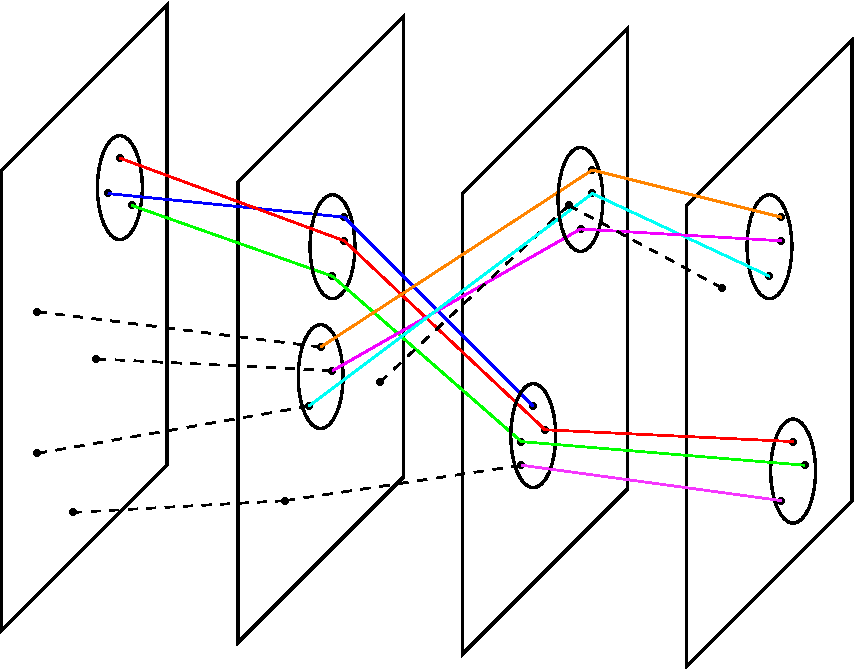
\includegraphics[width=0.55\textwidth]{figures/flock}

        \begin{itemize}
            \item $\varepsilon$: Maximum distance between objects.
            \item $\mu$: Minimum number of objects.
            \item $\delta$: Minimum time the objects keep `together'.
        \end{itemize}
    \end{frame}

    \begin{frame}{\textbf{B}asic \textbf{F}lock \textbf{E}valuation algorithm}
        \begin{itemize}
            \item Vieira, et al. 2009.
            \item The first polynomial-time solution for determining disk locations.
            \item Under fixed time duration it has polynomial time complexity $O(\delta|\tau|^{(2\delta) + 1})$
        \end{itemize}
        \vspace{0.25cm}

        \centering
        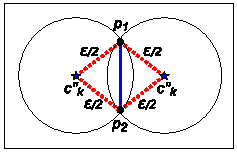
\includegraphics[width=0.4\textwidth]{figures/theorem}

    \end{frame}

    \begin{frame}{\textbf{B}asic \textbf{F}lock \textbf{E}valuation algorithm}
        \begin{itemize}
            \item Two main parts:
            \begin{itemize}
                \item In the spatial domain it finds maximal disks at each time stamp.
                \item In the temporal domain it joins consecutive times to match set of maximal disks.
            \end{itemize}
        \end{itemize}
    \end{frame}

    \begin{frame}{On the spatial domain}
        \begin{itemize} \item BFE overview... \end{itemize} \vspace{0.5cm}

        \centering
        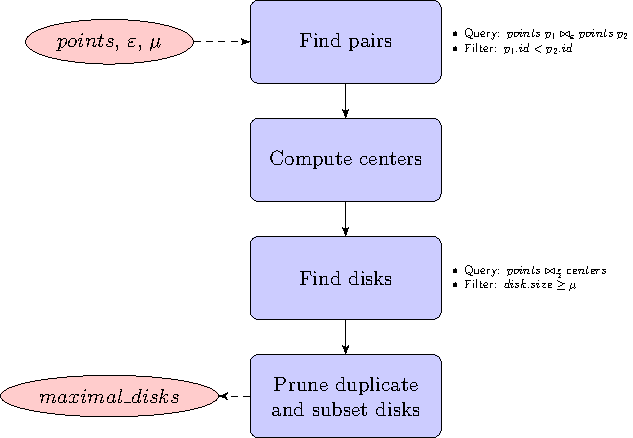
\includegraphics[width=0.7\textwidth]{../thesis/chapter4/figures/MF_flowchart}
    \end{frame}

    \begin{frame}{On the spatial domain}
        \begin{itemize} \item BFE overview... \end{itemize} \vspace{0.5cm}

        \centering
        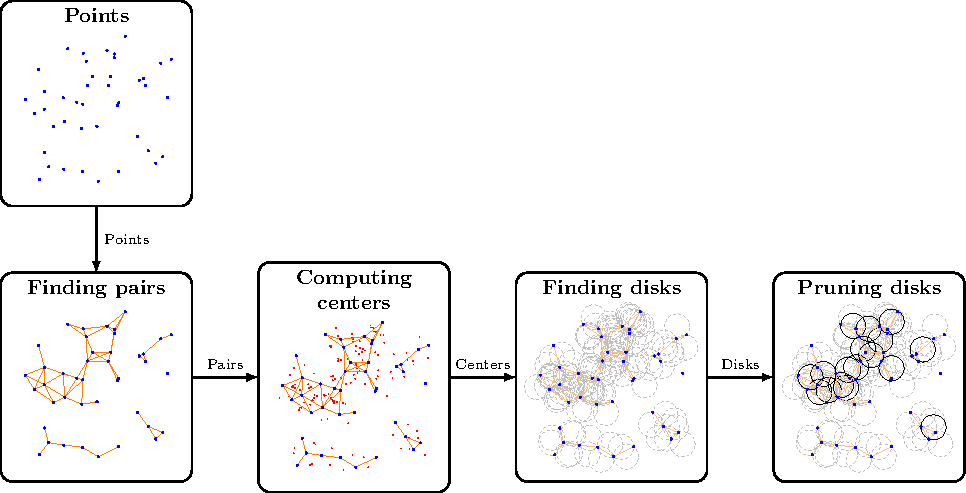
\includegraphics[width=\textwidth]{../thesis/chapter4/figures/MF_stages2/flow}
    \end{frame}

    \begin{frame}{On the temporal domain}
        \begin{itemize} \item BFE overview... \end{itemize} \vspace{0.5cm}

        \centering
        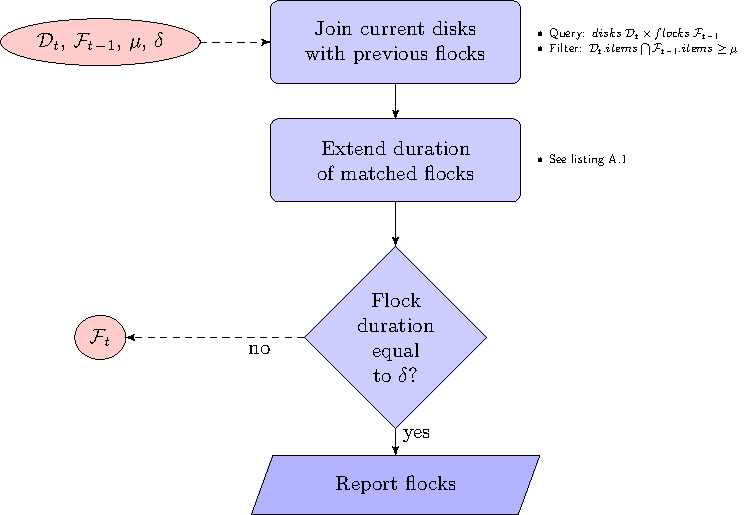
\includegraphics[width=0.7\textwidth]{../thesis/chapter4/figures/FF_flowchart}
    \end{frame}

    \begin{frame}{On the temporal domain}
        \begin{itemize} \item BFE overview... \end{itemize} \vspace{0.5cm}

        \centering
        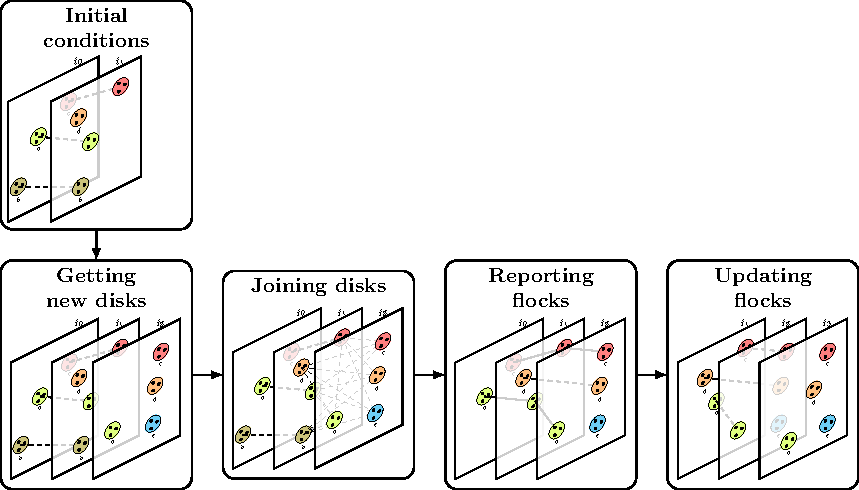
\includegraphics[width=\textwidth]{../thesis/chapter4/figures/Temporal/f_stages}
    \end{frame}

    \begin{frame}{PSI algorithm}
        \begin{minipage}{0.5\textwidth}
            \centering
            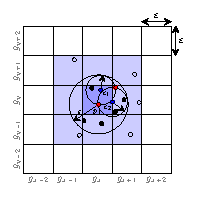
\includegraphics[width=\textwidth]{../thesis/chapter4/figures/grid_prime}
        \end{minipage}\hfill % maximize the horizontal separation
        \begin{minipage}{0.5\textwidth}
            \vspace{6mm}
            \centering
            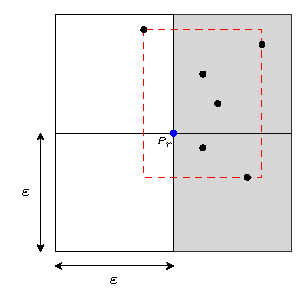
\includegraphics[width=0.78\textwidth]{../thesis/chapter4/figures/square}
        \end{minipage}
    \end{frame}


    \begin{frame}{Challenges and contributions}
        \begin{itemize}
            \item Due to high complexity it does not scale well.
            \item In databases with a large number of moving entities per time stamp it has a direct impact.
            \item Just sequential implementation yet.
            \item We propose a parallel solution in both domains.
        \end{itemize}
    \end{frame}

    \begin{frame}{On the spatial domain}{}
        \begin{itemize} \item Parallel overview... \end{itemize} \vspace{0.5cm}

         \centering
         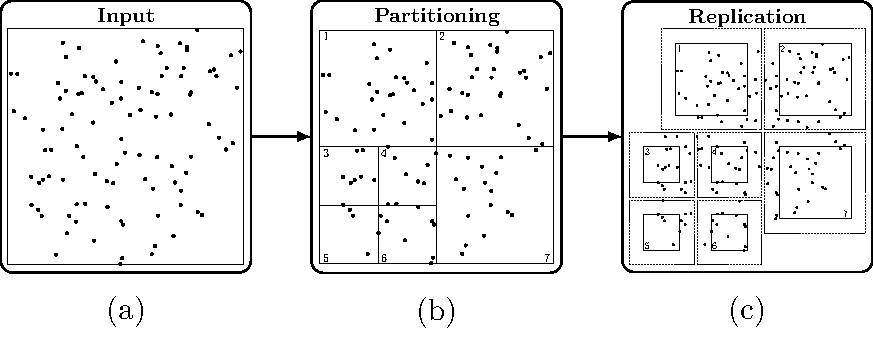
\includegraphics[width=\textwidth]{../thesis/chapter4/figures/PartReplication/P123}
     \end{frame}

     \begin{frame}{On the spatial domain}
        \begin{itemize} \item Parallel overview... \end{itemize} \vspace{0.5cm}

         \centering
         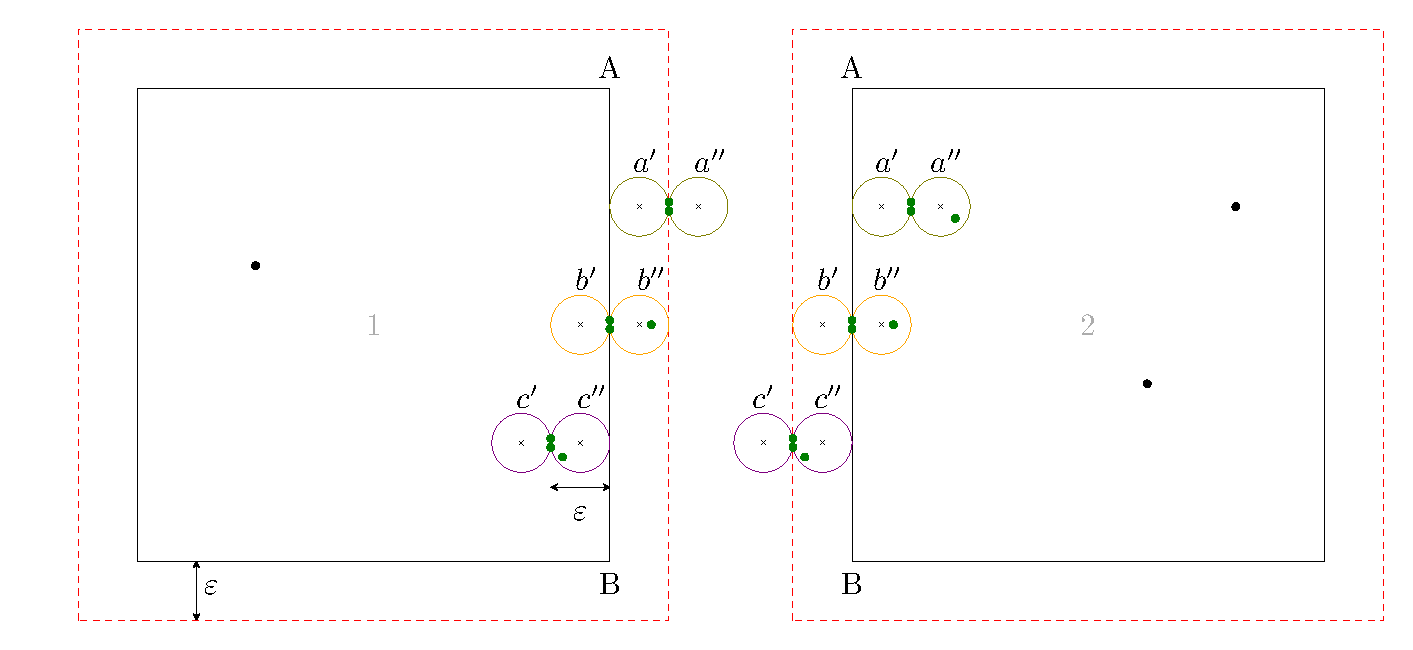
\includegraphics[width=\textwidth]{../thesis/chapter4/figures/merge}
     \end{frame}

    \begin{frame}{On the temporal domain}
        \centering
        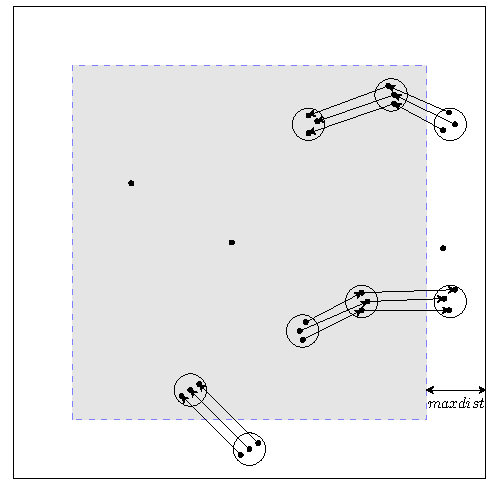
\includegraphics[height=0.75\textheight]{../thesis/chapter4/figures/maxdist}
    \end{frame}

    \begin{frame}{On the temporal domain}
        \centering
        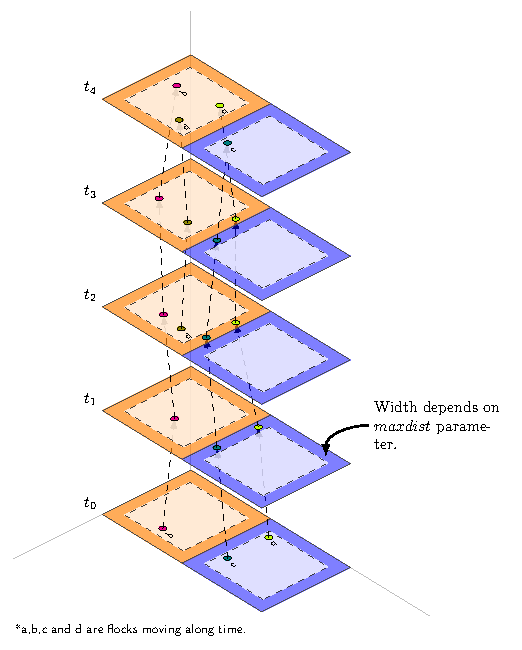
\includegraphics[height=0.9\textheight]{../thesis/chapter4/figures/plots/11_temporal_partitions/TemporalPartitioning}
    \end{frame}

    \begin{frame}{On the temporal domain}
        \centering
        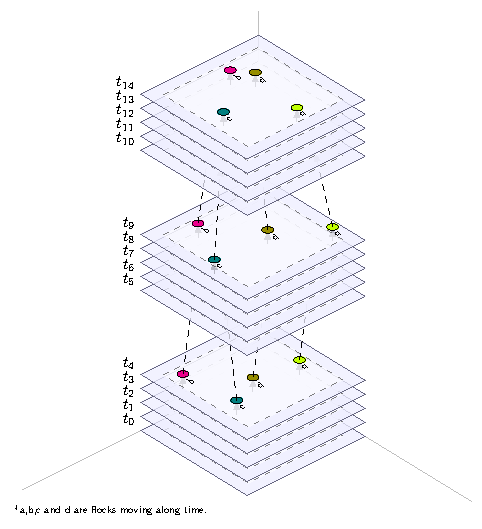
\includegraphics[height=0.9\textheight]{../thesis/chapter4/figures/plots/11_temporal_partitions/Cube-based}
    \end{frame}

    \begin{frame}{Datasets}
            \centering
            \begin{tabular}{cccc}
                \hline
                        & Number of    & Total number & Maximum        \\
                Dataset & Trajectories & of points    & Duration (min) \\
                \hline
                Berlin10K &  10000 & 97526 & 10\\
                LA25K &  25000 & 1495637 & 30\\
                LA50K &  50000 & 2993517 & 60\\
                \hline
            \end{tabular}
     \end{frame}

     \begin{frame}{Datasets}
        \begin{itemize} \item Synthetic dataset [LA: 50K objects]\end{itemize} \vspace{0.25cm}

         \centering
         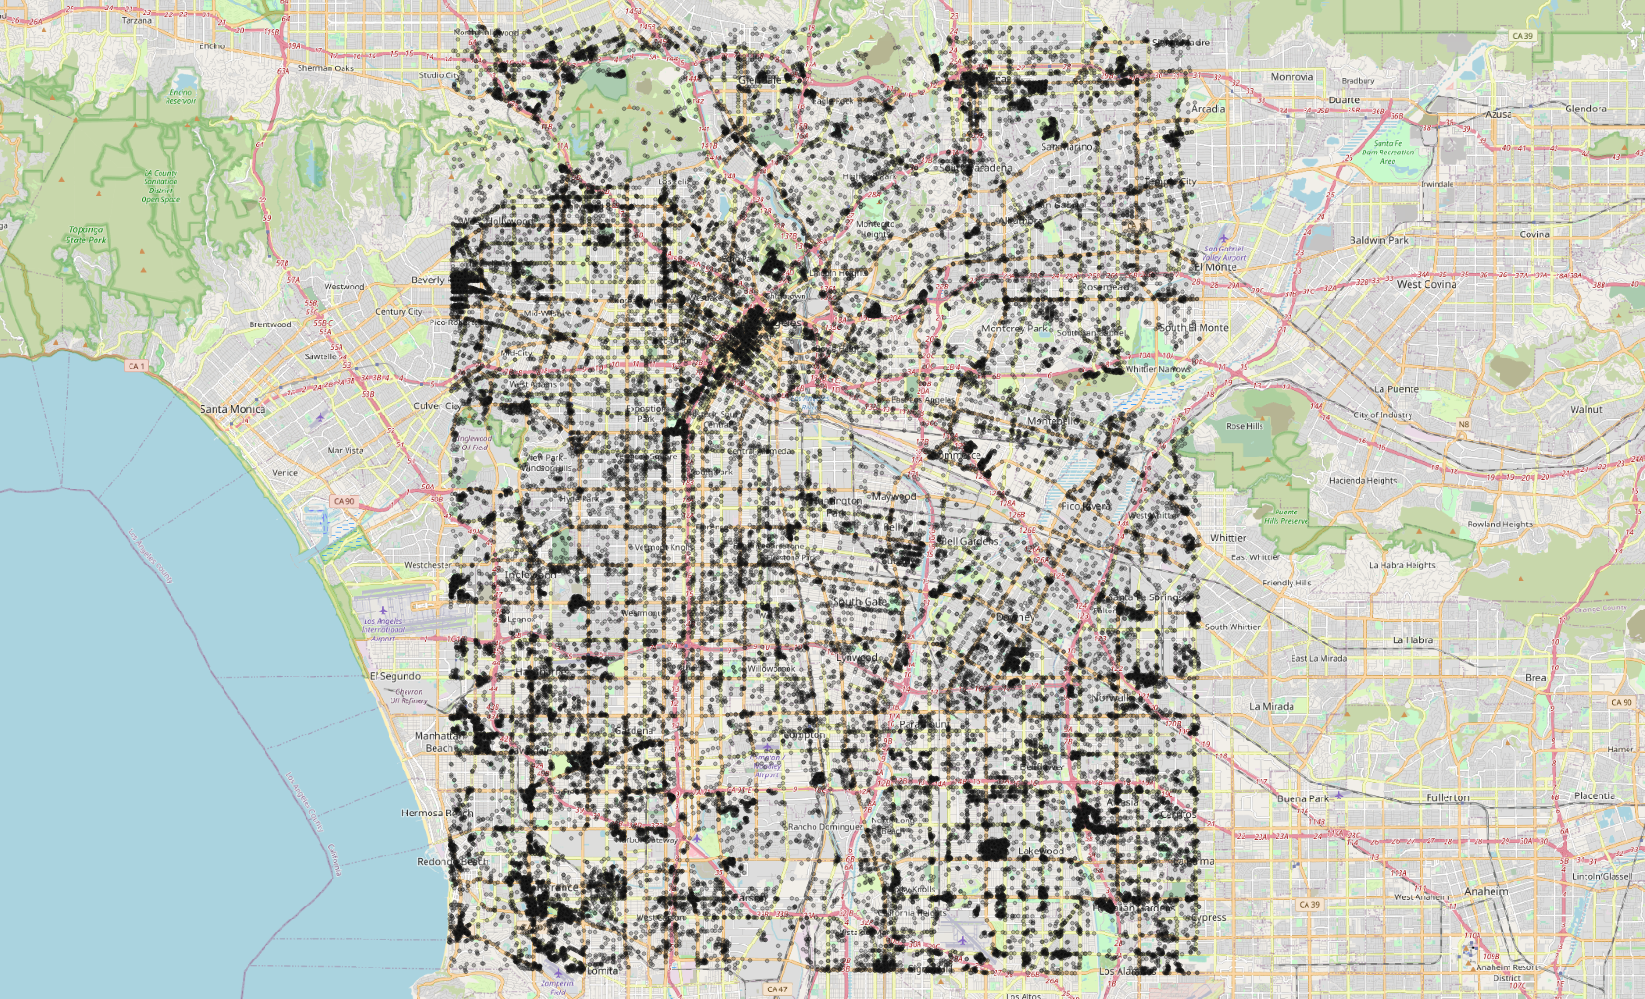
\includegraphics[width=\textwidth]{figures/LA_T320_N50K.png}
     \end{frame}

    \begin{frame}{Experiments}
        \begin{itemize} \item Optimizing the number of partitions for Phase 1. \end{itemize} \vspace{0.5cm}

        \begin{figure}
            \centering
            \begin{subfigure}[t]{0.32\textwidth}
                \raisebox{-\height}{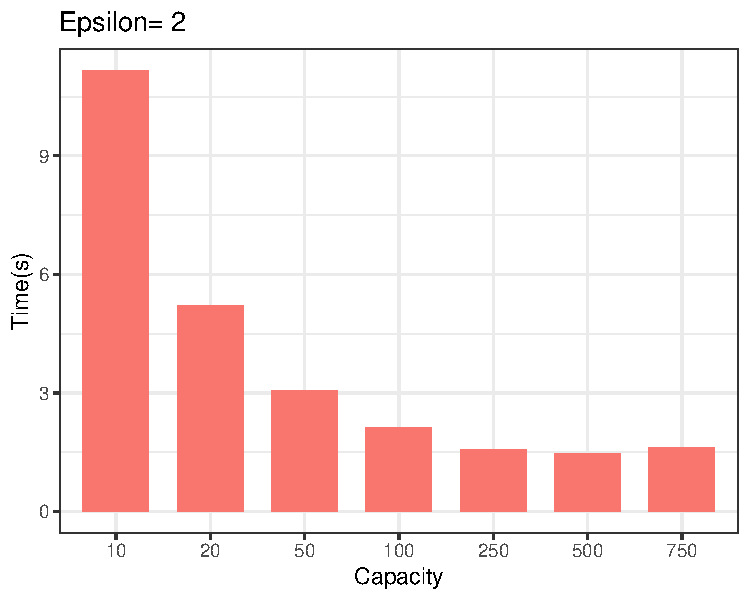
\includegraphics[width=\textwidth]
                {../thesis/chapter4/figures/plots/01_optimal_performance/pflockE2_by_capacity}}
            \end{subfigure}
            \hfill
            \begin{subfigure}[t]{0.32\textwidth}
                \raisebox{-\height}{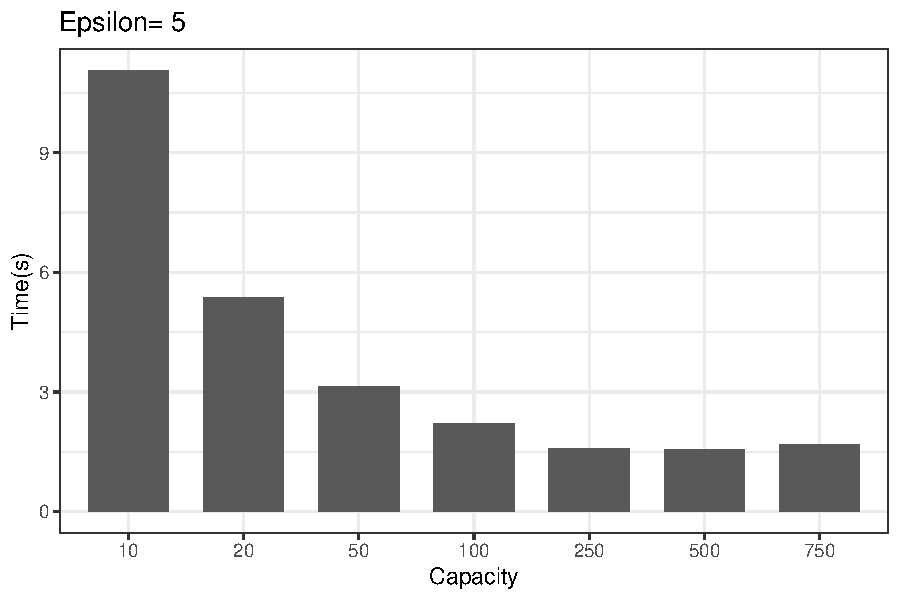
\includegraphics[width=\textwidth]
                {../thesis/chapter4/figures/plots/01_optimal_performance/pflockE5_by_capacity}}
            \end{subfigure}
            \hfill
            \begin{subfigure}[t]{0.32\textwidth}
                \raisebox{-\height}{\includegraphics[width=\textwidth]
                {../thesis/chapter4/figures/plots/01_optimal_performance/pflockE10_by_capacity}}
            \end{subfigure}
            %%%%%%%%%%%%%%%%%%%%%%%%%%%%%%%%%%%%second row
            \begin{subfigure}[t]{0.32\textwidth}
                \raisebox{-\height}{\includegraphics[width=\textwidth]
                {../thesis/chapter4/figures/plots/01_optimal_performance/pflockE15_by_capacity}}
            \end{subfigure}
            %\hfill
            \begin{subfigure}[t]{0.32\textwidth}
                \raisebox{-\height}{\includegraphics[width=\textwidth]
                {../thesis/chapter4/figures/plots/01_optimal_performance/pflockE20_by_capacity}}
            \end{subfigure}
        \end{figure}
    \end{frame}

    \begin{frame}{Experiments}
        \begin{itemize} \item Analyzing most costly partitions. \end{itemize} \vspace{0.5cm}
        \includegraphics[width=\textwidth]
                {../thesis/chapter4/figures/plots/03_top_time_partitions/top_time_partitions}

    \end{frame}

    \begin{frame}{Experiments}
        \centering
        \includegraphics[width=0.9\textwidth]
                {../thesis/chapter4/figures/plots/04_pairs_performance/pairs_performance}
    \end{frame}

    \begin{frame}{Experiments}
        \centering
        \includegraphics[width=\textwidth]
                {../thesis/chapter4/figures/plots/09_dense_stages/dense}
    \end{frame}

    \begin{frame}{Experiments}
        \centering
        \includegraphics[width=\textwidth]
                {../thesis/chapter4/figures/plots/10_cmbc_variants/cmbc}
    \end{frame}

    \begin{frame}{Experiments}
        \centering
        \includegraphics[width=0.9\textwidth]
                {../thesis/chapter4/figures/plots/05_uniform_performance/uniform_performance}
    \end{frame}

    \begin{frame}{Experiments}
        \centering
        \includegraphics[width=0.9\textwidth]
                {../thesis/chapter4/figures/plots/06_step_performance/step_performance}
    \end{frame}

    \begin{frame}{Experiments}
        \centering
        \includegraphics[width=0.9\textwidth]
                {../thesis/chapter4/figures/plots/07_interval_performance/interval-performance}
    \end{frame}

    \begin{frame}{Experiments}
        \centering
        \includegraphics[width=0.9\textwidth]
                {../thesis/chapter4/figures/plots/08_sequential_parallel/la25k_e_bfe_psi}
    \end{frame}

    \begin{frame}{Experiments}
        \centering
        \includegraphics[width=0.9\textwidth]
                {../thesis/chapter4/figures/plots/08_sequential_parallel/la25k_e}
    \end{frame}

    \begin{frame}{Experiments}
        \centering
        \includegraphics[width=0.9\textwidth]
                {../thesis/chapter4/figures/plots/08_sequential_parallel/la50k_e}
    \end{frame}

    \begin{frame}{ \ }
        \LARGE Thank you!
    \end{frame}
\end{document}
